\documentclass{ctexart}

\usepackage{bm}
\usepackage{geometry}
\usepackage{titlesec} %自u格式的宏包
\usepackage{picinpar,graphicx}
\usepackage{zhnumber}
\usepackage{float}
\usepackage{caption,subcaption}
\usepackage{amsmath}
\usepackage{amssymb}
\usepackage{fancyhdr}%页眉页脚
\usepackage{multirow}
\usepackage{upgreek}
\usepackage{paralist}
\usepackage{diagbox,array}

\geometry{a4paper,left=0.75in,right=0.75in,top=1in,bottom=1in} %页边距


\counterwithin{figure}{section}
\counterwithin{table}{section}

\renewcommand{\thefigure}{ \arabic{section}-\arabic{figure}}
\renewcommand{\thetable}{ \arabic{section}-\arabic{table}}
\renewcommand \thesubsection {(\zhnum{section})}
\renewcommand{\caption}[1]{\caption[\songti\ziju{-5}]{#1}}
%\\totalnumber{10}
%\renewcommand{\thesubfigure}{\arabic{section}-\arabic{figure}-\arabic{subfigure}}

\titleformat{\section}[block]{\zihao{3}\bfseries}{\zhnum{section}、}{1em}{}[]
\titleformat{\subsection}[block]{\zihao{-3}\mdseries}{(\zhnum{subsection})}{1em}{}[]
\titleformat{\subsubsection}[block]{\zihao{4}\bfseries}{\arabic{subsubsection}.}{1em}{}[]
%%\titleformat{\paragraph}[block]{\songti\zihao{5}}{[\arabic{paragraph}]}{1em}{}[]

\setlength{\baselineskip}{20pt}

\pagestyle{plain}
\pagenumbering{arabic}
\zihao{-4}
\setlength{\parskip}{0.1pt}
\begin{document}
	
	\section{引言}
		本文通过误差理论与数据处理的相关手段，对测得电压和电流进行了统计分析，并使用最小二乘法作出了对电阻值的估计。
	\section{研究内容}
		研究大致基于以下内容展开：
		\begin{enumerate}
			\item 测量了两组不同精度下的同一电压值，对每组数据做等精度处理后，对两次统计结果作不等精度数据处理，得出最终结果。
			\item 测量了两组不同精度下的同一电流值，对每组数据做等精度处理后，对两次统计结果作不等精度数据处理，得出最终结果。
			\item 测量了一组同精度下的不同一电压值，及对应等进度电流值，通过最小二乘法的手段进行求值运算，得出未知电阻$R_x$及电压表电流$I_u$的估算值。
		\end{enumerate}
	\section{研究流程}
		研究大致分为四个步骤，其研究流程如图\ref{fig:实验流程图}：
		\begin{enumerate}
			\item 设计实验，绘制对应测试电路图，得到实验电路板。
			\item 根据实验预先设计，进行数据测量。
			\item 不改变电位器电阻值下，等精度测量各两组电压和电流值，等进度处理后，作不等精度处理。
			\item 改变电位器电阻后，测量多组电压电流的对应值，并进行最小二乘法处理。
		\end{enumerate}
		\begin{figure}[h]
			\centering
			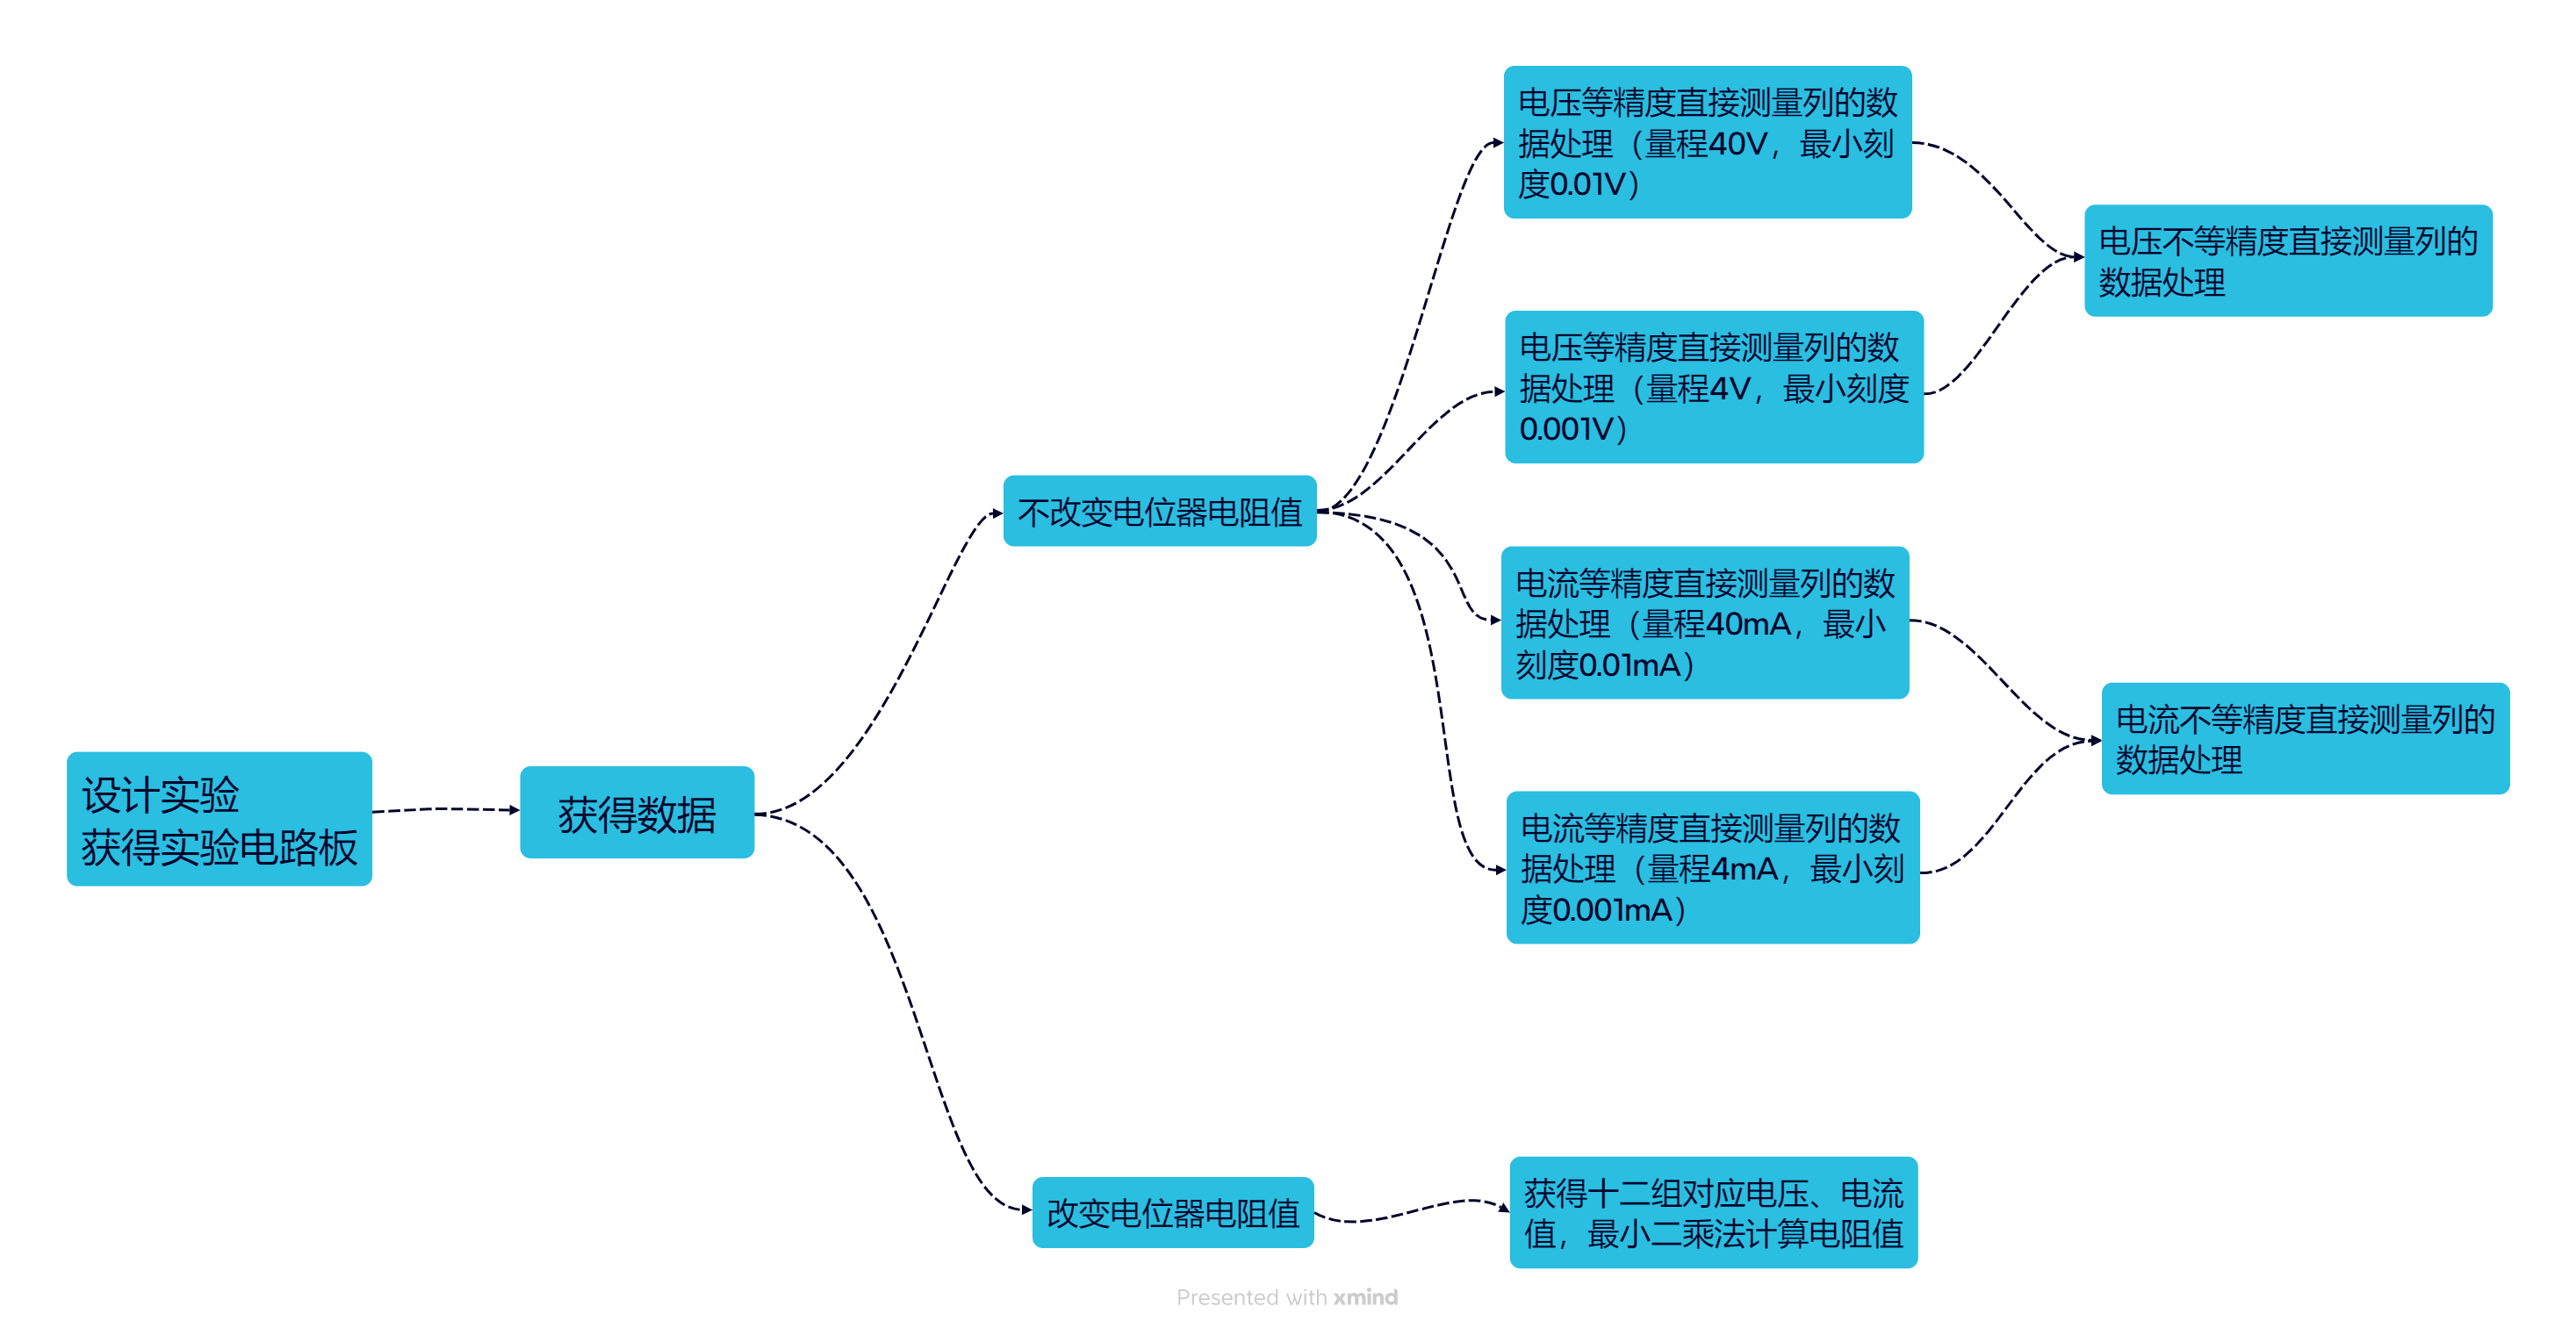
\includegraphics[width=0.45\textwidth]{../截图/获得数据}
			\caption{实验流程图}
			\label{fig:实验流程图}
		\end{figure}
		\subsection{设计实验}
			经过小组讨论后，最终确认本次实验围绕电学物理实验——“伏安法测电阻”进行。\par
			伏安法（又称伏特测量法、安培测量法）是一种较为普遍的测量电阻的方法，通过利用部分电路欧姆定律：$R=\frac{U}{I}$来测出电阻值。用电流表测出在此电压下通过未知电阻的电流，然后计算出未知电阻的阻值，这种测电阻的方法，叫伏安法。\par
			基于伏安法的实验原理，可以得到实验原理图（如图\ref{fig:伏安法测电阻实验原理图}）。
			\begin{figure}[h]
				\centering
				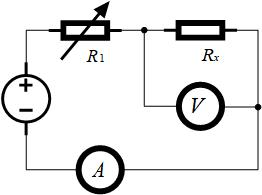
\includegraphics[width=0.45\textwidth]{../截图/电路原理图}
				\caption{伏安法测电阻实验原理图}
				\label{fig:伏安法测电阻实验原理图}
			\end{figure}
			本次实验，采用电流表外接的形式。因此需要在后续进行数据处理时考虑电压表内阻通过的电流，对实验的影响。\par
			根据实验原理图，便可以设计实际原理图和电路板。
			\begin{figure}[h]
				\centering
				\begin{subfigure}{0.325\linewidth}
					\centering
					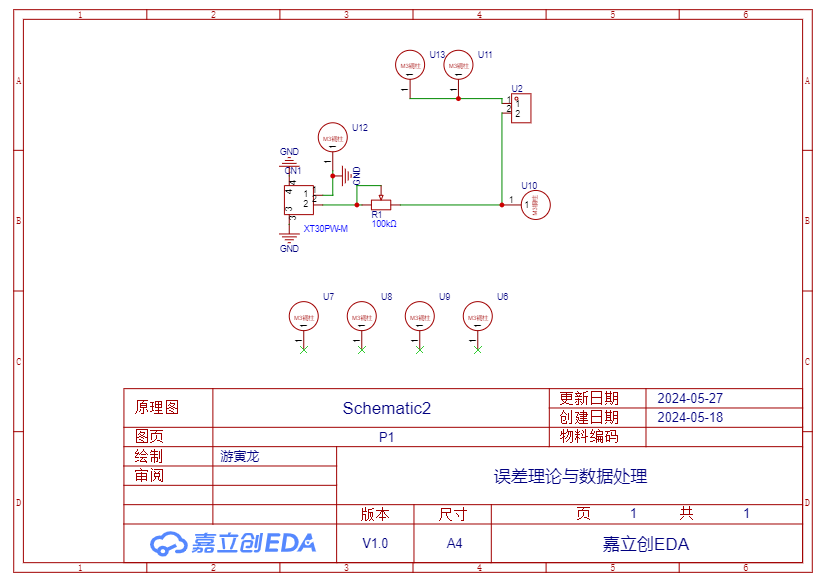
\includegraphics[width=0.9\linewidth]{../截图/电路板原理图}
					\caption{实验电路板原理图}
				\end{subfigure}
				\centering
				\begin{subfigure}{0.325\linewidth}
					\centering
					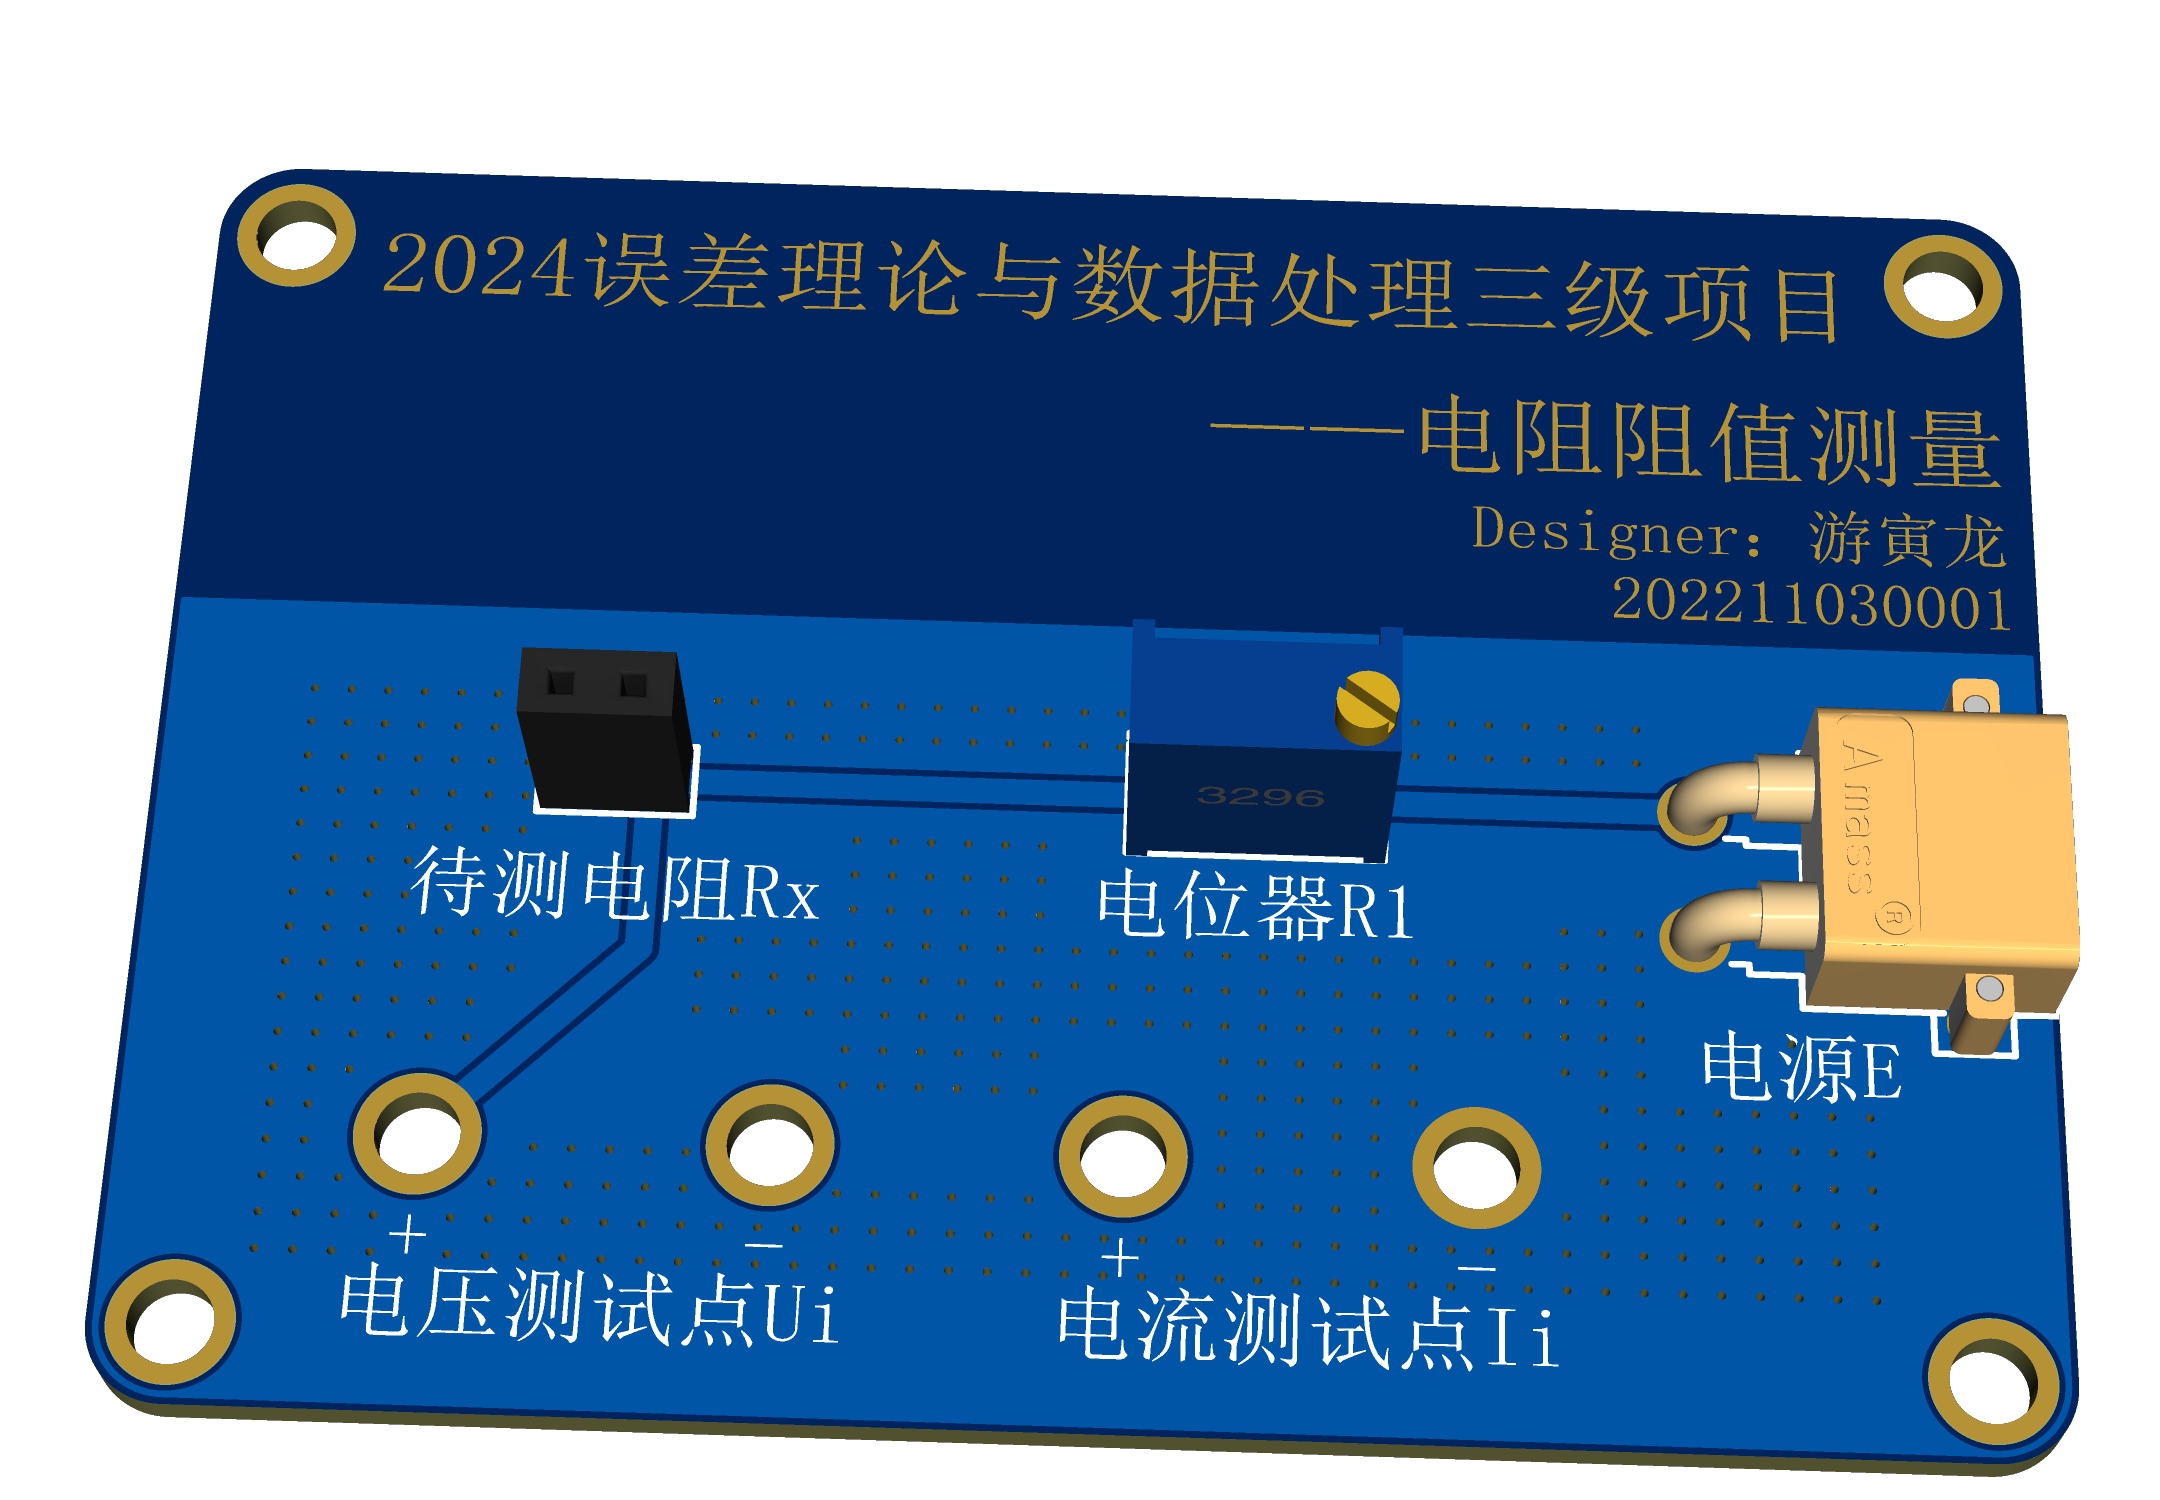
\includegraphics[width=0.9\linewidth]{../截图/电路板3D仿真图}
					\caption{实验电路板仿真图}
				\end{subfigure}
				\centering
				\begin{subfigure}{0.325\linewidth}
					\centering
					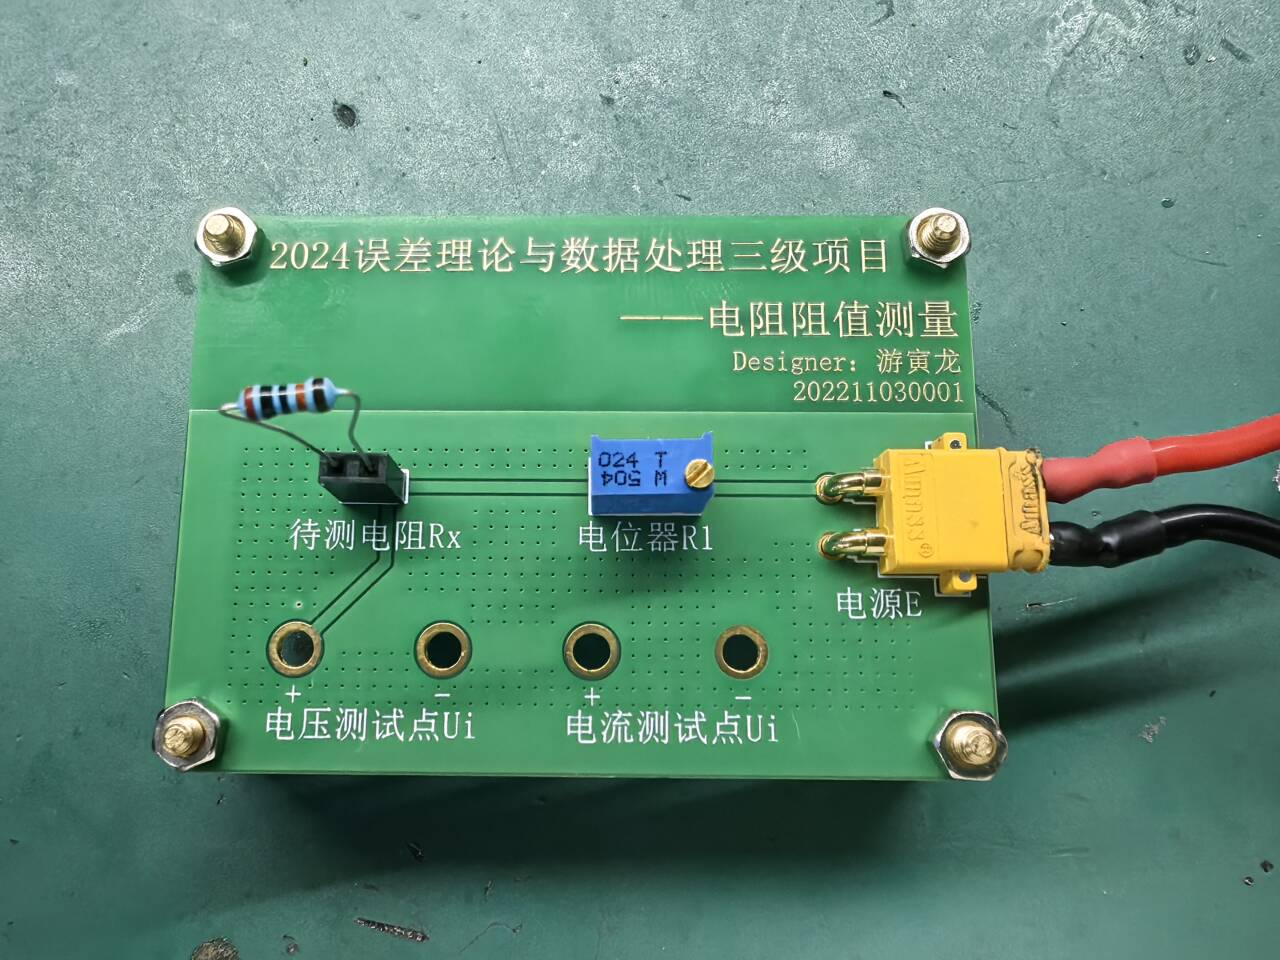
\includegraphics[width=0.9\linewidth]{../截图/电路板实际图}
					\caption{实验电路板实际图}
				\end{subfigure}
				\caption{伏安法测电阻实验电路板}
				\label{fig:伏安法测电阻实验电路板}
			\end{figure}
		\subsection{数据测量}
			测量使用两个同样型号（型号：LCSC530+）的万用表进行，实际测量方式如图\ref{fig:伏安法测电阻实验测量方式}。
			
			其中，左侧表作为电压表使用，测量电压；右侧表作为电流表使用，测量电流。\par
			\begin{figure}[h]
				\centering
				\begin{subfigure}{0.325\linewidth}
					\centering
					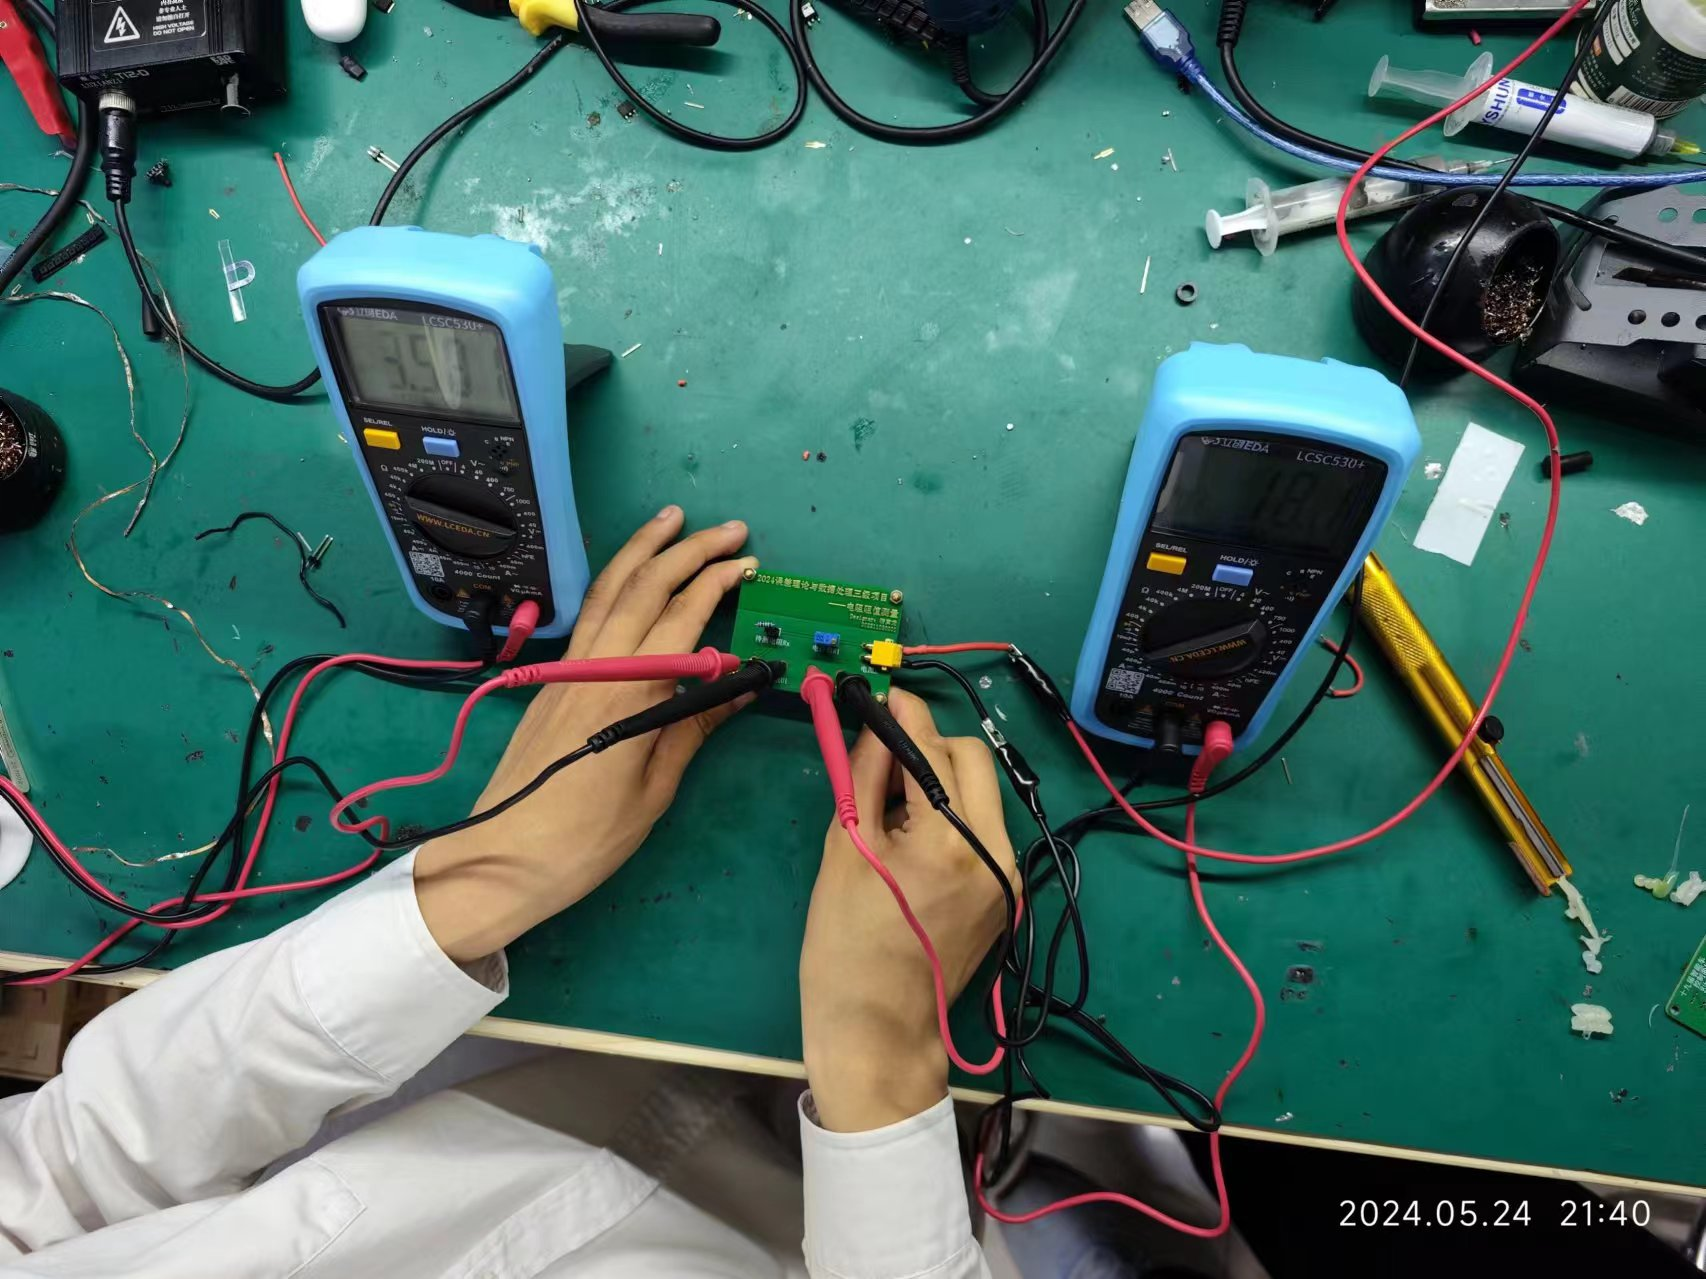
\includegraphics[width=0.9\linewidth]{../截图/实际测量1}
				\end{subfigure}
				\centering
				\begin{subfigure}{0.325\linewidth}
					\centering
					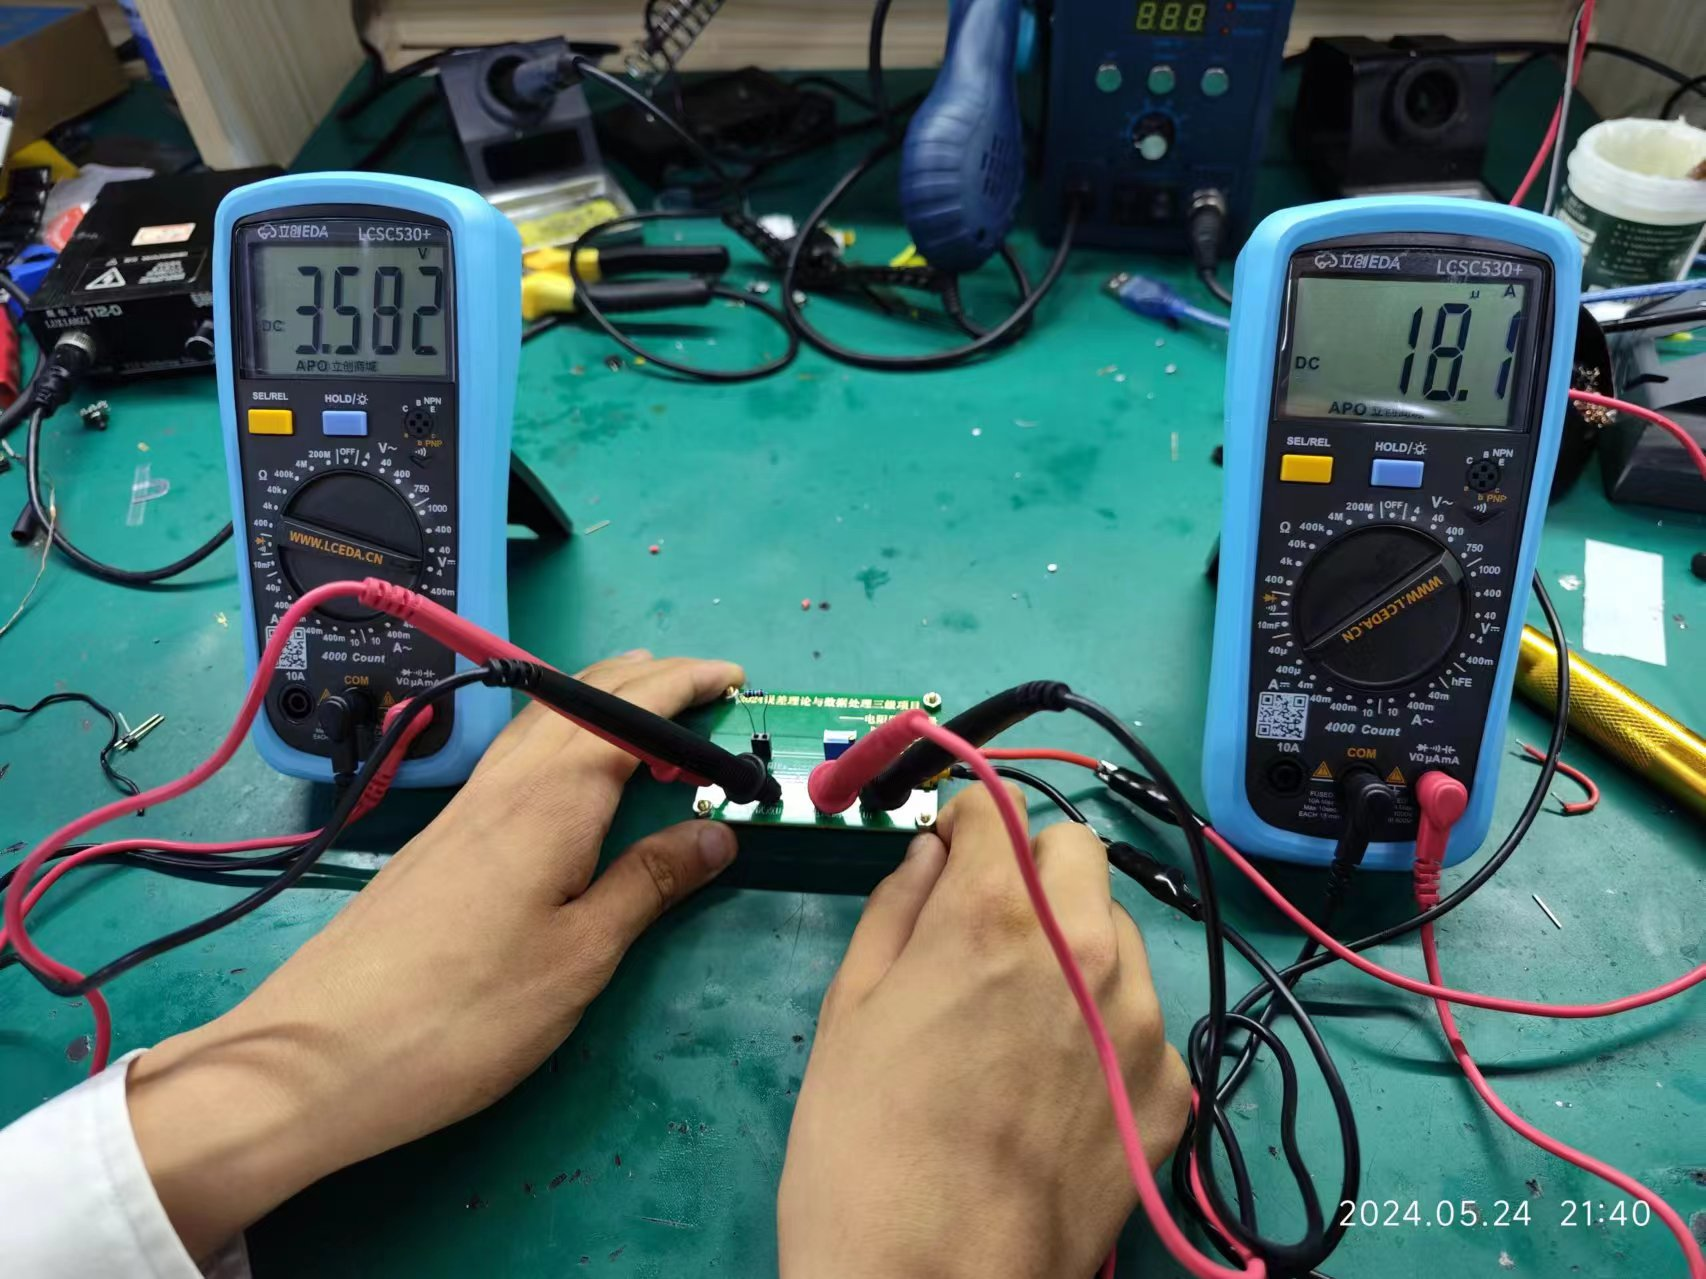
\includegraphics[width=0.9\linewidth]{../截图/实际测量2}
				\end{subfigure}
				\caption{伏安法测电阻实验测量方式}
				\label{fig:伏安法测电阻实验测量方式}
			\end{figure}
			首先进行等精度下的电压测量。\par
			使用量程为40V，最小分度值为0.01V的档位，测量电压数据如表\ref{fig:量程为40V、最小分度值为0.01V时电压采样数据}所示。\par
			\begin{table}[h]
				\centering
				\caption{量程为40V、最小分度值为0.01V时电压采样数据}
				\begin{tabular}{c c c c c c c}%r右对齐，c居中，l左对齐
					\hline
					次数 & 1&2&3&4&5&6\\
					\hline
					测量值（V）&3.57&3.58&3.58&3.58&3.58&3.57\\
					\hline
				\end{tabular}
				\label{fig:量程为40V、最小分度值为0.01V时电压采样数据}
			\end{table}
			使用量程为4V，最小分度值为0.001V的档位，测量电压数据如表\ref{fig:量程为4V、最小分度值为0.001V时电压采样数据}所示。\par
			\begin{table}[]
				\centering
				\caption{量程为4V、最小分度值为0.001V时电压采样数据}
				\begin{tabular}{c c c c c c c c c c}%r右对齐，c居中，l左对齐
					\hline
					次数 & 1&2&3&4&5&6&7&8&9\\
					\hline
					测量值（V）&3.578&3.580&3.582&3.580&3.577&3.583&3.586&3.579&3.584\\
					\hline
				\end{tabular}
				\label{fig:量程为4V、最小分度值为0.001V时电压采样数据}
			\end{table}
			随后进行等精度下的电流测量。\par
			使用量程为400$\upmu$A，最小分度值为0.1$\upmu$A的档位，测量电流数据如表\ref{fig:量程为400uA，最小分度值为0.1uA时电流采样数据}所示。\par
			\begin{table}[H]
				\centering
				\caption{量程为400$\upmu$A，最小分度值为0.1$\upmu$A时电流采样数据}
				\begin{tabular}{c c c c c c c}%r右对齐，c居中，l左对齐
					\hline
					次数 & 1&2&3&4&5&6\\
					\hline
					测量值（$\upmu$A）&18.0&18.1&18.1&18.0&18.1&18.0\\
					\hline
				\end{tabular}
				\label{fig:量程为400uA，最小分度值为0.1uA时电流采样数据}
			\end{table}
			使用量程为40$\upmu$A，最小分度值为0.01$\upmu$A的档位，测量电流数据如表\ref{fig:量程为40uA，最小分度值为0.01uA时电流采样数据}所示。\par
			\begin{table}[H]
				\centering
				\caption{量程为40$\upmu$A，最小分度值为0.01$\upmu$A时电流采样数据}
				\begin{tabular}{c c c c c c c c c c}%r右对齐，c居中，l左对齐
					\hline
					次数 & 1&2&3&4&5&6&7&8&9\\
					\hline
					测量值（$\upmu$A）&18.09&18.09&18.09&18.08&18.09&18.09&18.08&18.09&18.08\\
					\hline
				\end{tabular}
				\label{fig:量程为40uA，最小分度值为0.01uA时电流采样数据}
			\end{table}
			最后对电位器电阻进行改变，测得多组电压电流的对应值。\par
			其中，电压档选用量程为4V、最小分度值为0.001V，电流档选用量程为40$\upmu$A，最小分度值为0.01$\upmu$A。测量结果如表\ref{fig:伏安法测电阻采样数据}所示。
			\begin{table}[H]
				\centering
				\caption{量程为40$\upmu$A，最小分度值为0.01$\upmu$A时电流采样数据}
				\begin{tabular}{cc c c c c c c c}
					\hline
					次数 & 1&2&3&4&5&6&7&8\\
					\hline
					电压测量值（V） &0.530&0.569&1.013&1.822&1.824&2.058&2.557&2.701\\
					电流测量值（$\upmu$A）&2.83&3.01&5,25&9.33&9.36&10.49&13.00&13.73\\
					\hline\hline
					次数&9&10&11&12&13&14&15&16\\
					\hline
					电压测量值（V）&3.039&3.920&4.610&4.765&4.811&5.644&6.181&6.186\\
					电流测量值（$\upmu$A）&15.42&19.86&23.34&24.12&24.34&28.54&31.24&31.29\\
					\hline
				\end{tabular}
				\label{fig:伏安法测电阻采样数据}
			\end{table}
		\subsection{数据处理}
			首先针对表\ref{fig:量程为40V、最小分度值为0.01V时电压采样数据}、表\ref{fig:量程为4V、最小分度值为0.001V时电压采样数据}、表\ref{fig:量程为400uA，最小分度值为0.1uA时电流采样数据}、表\ref{fig:量程为40uA，最小分度值为0.01uA时电流采样数据}中的四次数据进行等精度处理。\par
			随后针对表\ref{fig:量程为40V、最小分度值为0.01V时电压采样数据}和表\ref{fig:量程为4V、最小分度值为0.001V时电压采样数据}等精度处理后的电压值、表\ref{fig:量程为400uA，最小分度值为0.1uA时电流采样数据}、表\ref{fig:量程为40uA，最小分度值为0.01uA时电流采样数据}等精度处理后的电流值，进行不等精度数据处理。\par
			最后针对表\ref{fig:伏安法测电阻采样数据}中的数据进行最小二乘法估算电阻值。\par
			其详细过程将在后续陈述。
	\section{理论原理}
		以下，对于《误差理论与数据处理》一书中所述等精度数据处理方法做出简要叙述。
		\subsection{等精度数据处理}
			等精度测量数据处理是指在整个测量过程中，影响和决定误差大小的全部因素（条件）始终保持不变。\par
			等精度测量的数据处理分为九个步骤：
			\begin{inparaenum}
				\item 求算术平均值
				\item 求残余误差
				\item 校核算术平均值及其残余误差
				\item 判断系统误差
				\item 求测量列单次测量的标准差
				\item 判断粗大误差
				\item 求算术平均值的标准差
				\item 求算术平均值的极限误差
				\item 写出最后测量结果。
			\end{inparaenum}\par
			
			定义:等精度测量列为$l_i$。
			\subsubsection{求算术平均值}
				算术平均值指被测量的$n$个测得值的袋鼠和除以$n$而得的值。根据定义，算术平均值$\bar{x}$的计算方法为：
				\begin{gather}
					\bar{x} =\frac{l_1+l_2+\cdots+l_n}{n}= \frac{\sum \limits_{i=1} ^{n} l_i}{n} 
					\label{fig:算术平均值公式}
				\end{gather}
			\subsubsection{求残余误差}
				残余误差指测得值与真值之间的差值。由于真值一般无法得到，因此使用最接近真值的算术平均值$\bar{x}$代替真值。据此残余误差$v_i$的计算方法为：
				\begin{gather*}
					v_i=l_i - \bar{x}\qquad i = 1,2,\cdots,n
				\end{gather*}
			\subsubsection{校核算术平均值及其残余误差}
				算术平均值及其残余误差的计算是否正确，可用求得的残余误差代数和的性质来校核。其有两个可行的规则。
				\paragraph{规则一}
					残余误差代数和应满足：
					\begin{compactitem}
						\item 当$\sum \limits_{i=1}^n l_i=n\bar{x}$，求得的$\bar{x}$为非凑整的准确数时，$\sum \limits_{i=1}^n v_i$为零
						\item 当$\sum \limits_{i=1}^n l_i>n\bar{x}$，求得的$\bar{x}$为凑整的非准确数时，$\sum \limits_{i=1}^n v_i$为正，其大小为求$\bar{x}$的余数
						\item 当$\sum \limits_{i=1}^n l_i<n\bar{x}$，求得的$\bar{x}$为凑整的非准确数时，$\sum \limits_{i=1}^n v_i$为负，其大小为求$\bar{x}$的亏数
					\end{compactitem}
				\paragraph{规则二}
					残余误差代数和绝对值应符合：
					\begin{compactitem}
						\item 当$n$为偶数时，$\Bigl| \sum \limits_{i=1}^n v_i \Bigl| \leq \frac{n}{2}A$
						\item 当$n$为奇数时，$\Bigl| \sum \limits_{i=1}^n v_i \Bigl| \leq (\frac{n}{2}-0.5)A$
					\end{compactitem}
					式中的$A$为实际求得的算术平均值$\bar{x}$末位数的一个单位。
			\subsubsection{判断系统误差}
				判断等精度测量系统误差共具有四种方法：
				\begin{inparaenum}
					\item 实验对比法
					\item 残余误差观察法
					\item 残余误差校核法
					\item 不同公式计算标准差比较法。
				\end{inparaenum}
				由于前两种方法过于主观，不具有计算可行性，故只说明后续两种方法。
				\paragraph{残余误差校核法(马利科夫准则)}
					将测量列中前$K$个残余误差相加，后$(n-K)$个残余误差相加，两者相减。当$n$为偶数，取$K=\frac{n}{2}$；当$n$为偶数，取$K=\frac{n+1}{2}$。公式表达如下：
					\begin{gather*}
						\Delta=\sum \limits_{i=1}^K v_i-\sum \limits_{j=K+1}^n v_j  \approx \sum \limits_{i=1}^{K} (l_{i}-\Delta \bar{x})-\sum \limits_{j=K+1}^{n}(l_{j}-\Delta \bar{x})
					\end{gather*}
					如果两部分的差值$\Delta$显著不为零，则可认为测量列存在线性系统误差。
				\paragraph{不同公式计算标准差比较法}
					本方法需要使用式\ref{con：贝塞尔公式}的贝塞尔公式所算出的标准差$\sigma$和式\ref{con：别捷尔斯公式}的别捷尔斯公式所算出的标准差$\sigma'$。\\
					令
					\begin{gather*}
						\frac{\sigma'}{\sigma}=1+u
					\end{gather*}
					若
					\begin{gather*}
						\lvert u \rvert \geq \frac{2}{\sqrt{n-1}}
					\end{gather*}
					则怀疑测量列中存在系统误差。
			\subsubsection{求测量列单次测量的标准差}
				测量列的标准偏差简称为标准差，也称之为方均根误差。\par
				求测量列单次测量的标准差共具有四种方法：
				\begin{inparaenum}
					\item 贝塞尔公式
					\item 别捷尔斯法
					\item 极差法
					\item 最大误差法。
				\end{inparaenum}\par
				由于最大误差法精度较低，不适用于本实验，便没有采用。
				\paragraph{贝塞尔公式}
					\begin{equation}
						\sigma=\sqrt{\frac{\sum \limits_{i=1}^n v_i^2}{n-1}}
						\label{con：贝塞尔公式}
					\end{equation}
				\paragraph{别捷尔斯法}
					\begin{equation}
						\sigma'=1.253\frac{\sum \limits_{i=1}^{n}\lvert v_{i} \rvert}{\sqrt{n(n-1)}}
						\label{con：别捷尔斯公式}
					\end{equation}
				\paragraph{极差法}
					若等精度多次测量测得值$l_1,l_2,\cdot,l_n$服从正态分布，在其中选取最大值$l_{max}$与最小值$l_{min}$，则两者之间的差称为极差，即
					\begin{gather*}
						\omega_n=l_{max}-l_{min}
					\end{gather*}
					标准差$\sigma$计算方式为
					\begin{gather*}
						\sigma=\frac{\omega_n}{d_n} 
					\end{gather*}
					式中，$d_n$的数值见表\ref{fig:极差系数表}
					\begin{table}[H]
						\centering
						\caption{极差系数表}
						\begin{tabular}{c| c c c c c c c c c c}
							\hline
							n &/&2&3&4&5&6&7&8&9&10\\
							\hline
							d &/&1.13&1.69&2.06&2.33&2.53&2.70&2.85&2.97&3.08\\
							\hline\hline
							n & 11&12&13&14&15&16&17&18&19&20\\
							\hline
							d &3.17&3.26&3.34&3.41&3.47&3.53&3.59&3.64&3.69&3.74\\
							\hline
						\end{tabular}
						\label{fig:极差系数表}
					\end{table}
			\subsubsection{判断粗大误差}
				粗大误差的数值比较大，会对测量结果产生明显的歪曲，一旦发现含有粗大误差的测量值，应将其从测量结果中剔除。\par
				判断粗大误差共具有四种方法：
				\begin{inparaenum}
					\item 3$\sigma$准则（莱以特准则）
					\item 罗曼诺夫斯基准则
					\item 格罗布斯准则
					\item 狄克松准则。
				\end{inparaenum}\par
				由于狄克松准则适用于测量次数少时的快速判断，不适用于本实验，便没有采用。
				\paragraph{3$\sigma$准则（莱以特准则）}
					若
					\begin{gather*}
						\lvert v_i \rvert >3\sigma
					\end{gather*}
					则可以认为它含有粗大误差，应当予以剔除。
				\paragraph{罗曼诺夫斯基准则}
					若认为测量值$l_j$为可疑数据，计算剔除可疑数据后的算术平均值和测量列的标准差
					\begin{gather*}
						\bar{x}' = \frac{1}{n-1} \sum \limits_{{i=1},{i \neq j}}^{n} l_i\\
						v_i'=l_i-\bar{x}' \qquad i=1,2,\cdots,j-1,j+1,\cdots,n\\
						\sigma'' = \sqrt{\frac{\sum \limits_{i=1}^{n} v_i^{'2}}{n-2}} 
					\end{gather*}
					根据测量次数$n$和选取的显著度$\alpha$，可由表\ref{fig:罗曼诺夫斯基系数表}查得$t$分布的检验系数$K(n,\alpha)$。\par
					若
					\begin{gather*}
						\lvert l_j-\bar{x}' \rvert >K \sigma''
					\end{gather*}
					则认为测量值$l_j$含有粗大误差，剔除$l_j$是正确的。
					\begin{table}[H]
						\centering
						\caption{罗曼诺夫斯基系数表}
						\begin{tabular}{c|c|c ||c| c |c||c| c |c}
							\hline
							\diagbox{$n$}{$K$}{$\alpha$} & 0.05 & 0.01 & \diagbox{$n$}{$K$}{$\alpha$} & 0.05 & 0.01 & \diagbox{$n$}{$K$}{$\alpha$} & 0.05 & 0.01\\
							\hline
							4 & 4.97 & 11.46 & 13 & 2.29 &3.23 & 22 & 2.14 &2.91\\ 
							 5 & 3.56 & 6.53 & 14 & 2.26 &3.17 & 23 & 2.13 &2.90\\ 
							 6 & 3.04 & 5.04 & 15 & 2.24 &3.12 & 24 & 2.12 &2.88\\ 
							 7 & 2.78 & 4.36 & 16 & 2.22 &3.08 & 25 & 2.11 &2.86\\ 
							 8 & 2.62 & 3.96 & 17 & 2.20 &3.04 & 26 & 2.10 &2.85\\ 
							 9 & 2.51 & 3.71 & 18 & 2.18 &3.01 & 27 & 2.10 &2.84\\ 
							10 & 2.43 & 3.54 & 19 & 2.17 &3.00 & 28 & 2.09 &2.83\\ 
							11 & 2.37 & 3.41 & 20 & 2.16 &2.95 & 29 & 2.09 &2.82\\ 
							12 & 2.33 & 3.31 & 21 & 2.15 &2.93 & 30 & 2.08 &2.81\\ 
							\hline
						\end{tabular}
						\label{fig:罗曼诺夫斯基系数表}
					\end{table}
				\paragraph{格罗布斯准则}
					根据式\ref{fig:算术平均值公式}所算的算术平均值和式\ref{con：贝塞尔公式}的贝塞尔公式所算的标准差$\sigma$。\\
					若认为$l_{max}$为可疑值，则计算
					\begin{gather*}
						g_{max}=\frac{\bar{x}-l_{max}}{\sigma}
					\end{gather*}
					若认为$l_{min}$为可疑值，则计算
					\begin{gather*}
						g_{min}=\frac{\bar{x}-l_{min}}{\sigma}
					\end{gather*}
					当
					\begin{gather*}
						g_i \geq g_0(n,\alpha)
					\end{gather*}
					即判别该测得值含有粗大误差，应当予以剔除。
					其中$g_0(n,\alpha)$根据测量次数$n$和选取的显著度$\alpha$，可由表\ref{fig:格罗布斯系数表}查得。
					\begin{table}[H]
						\centering
						\caption{格罗布斯系数表}
						\begin{tabular}{c|c|c ||c| c |c||c|c|c ||c| c |c}
							\hline
								\multicolumn{1}{c|}{\multirow{3}{*}{n}} &\multicolumn{2}{c||}{\multirow{1}{*}{$\alpha$}} & \multicolumn{1}{c|}{\multirow{3}{*}{n}} &\multicolumn{2}{c||}{\multirow{1}{*}{$\alpha$}}&
								\multicolumn{1}{c|}{\multirow{3}{*}{n}} &\multicolumn{2}{c||}{\multirow{1}{*}{$\alpha$}} & \multicolumn{1}{c|}{\multirow{3}{*}{n}} &\multicolumn{2}{c}{\multirow{1}{*}{$\alpha$}}\\
								\cline{2-3}\cline{5-6}\cline{8-9}\cline{11-12}
								\multicolumn{1}{c|}{\multirow{3}{*}{}}&0.05&0.01&\multicolumn{1}{c|}{\multirow{3}{*}{}}&0.05& 0.01&\multicolumn{1}{c|}{\multirow{3}{*}{}}&0.05&0.01&\multicolumn{1}{c|}{\multirow{3}{*}{}}&0.05& 0.01\\
								\cline{2-3}\cline{5-6}\cline{8-9}\cline{11-12}
								\multicolumn{1}{c|}{\multirow{3}{*}{}} &\multicolumn{2}{c||}{\multirow{1}{*}{$g_0(n,\alpha)$}} & \multicolumn{1}{c|}{\multirow{3}{*}{}} &\multicolumn{2}{c||}{\multirow{1}{*}{$g_0(n,\alpha)$}}&
								\multicolumn{1}{c|}{\multirow{3}{*}{}} &\multicolumn{2}{c||}{\multirow{1}{*}{$g_0(n,\alpha)$}} & \multicolumn{1}{c|}{\multirow{3}{*}{}} &\multicolumn{2}{c}{\multirow{1}{*}{$g_0(n,\alpha)$}}\\
							\hline
							3 &1.15&1.16&10&2.18&2.41&17&2.48&2.78&24&2.64&2.99\\
							4 &1.46&1.49&11&2.23&2.48&18&2.50&2.82&25&2.66&3.01\\
							5 &1.67&1.57&12&2.28&2.55&19&2.53&2.85&30&2.74&3.10\\
							6 &1.82&1.94&13&2.33&2.61&20&2.56&2.88&35&2.81&3.18\\
							7 &1.94&2.10&14&2.37&2.66&21&2.58&2.91&40&2.87&3.24\\
							8 &2.03&2.22&15&2.41&2.70&22&2.60&2.94&50&2.96&3.34\\
							9 &2.11&2.32&16&2.44&2.75&23&2.62&2.96&100&3,17&3.59\\
							\hline
						\end{tabular}
						\label{fig:格罗布斯系数表}
					\end{table}
			\subsubsection{求算术平均值的标准差}
				算术平均值的标准差$\sigma_{\bar{x}}$是表征同一被测量的各个独立测量列算术平均值分散性的参数。其计算公式为：
				\begin{gather*}
					\sigma_{\bar{x}}=\frac{\sigma}{\sqrt{n}}
				\end{gather*}
			\subsubsection{求算术平均值的极限误差}
				极限误差$\delta_{lim} \bar{x}$的表达式为：
				\begin{gather*}
					\delta_{lim} \bar{x}= \pm t_\alpha \sigma_{\bar{x}}
				\end{gather*}
				式中$t_\alpha$的取值方法有三种：
				\begin{compactenum}
					\item 一般直接取$t_\alpha=3$
					\item 若测量次数$n<10$，则按$t$分布计算。
					\item 若测量次数$n\geq 10$，则按正态分布计算。
				\end{compactenum}
			\subsubsection{写出最后测量结果}
				最后测量结果通常用算术平均值及其极限误差来表示，即
				\begin{gather*}
					L=\bar{x} \pm 	\delta_{lim} \bar{x}
				\end{gather*}
		\subsection{不等精度数据处理}
			在科学研究或高精度测量中，往往在不同的测量条件下，用不同的仪器、不同的测量方法、不同的测量次数以及不同的测量者进行测量与对比，这种测量称为不等精度测量。\par
			在一般测量工作中，常遇到的不等精度测量有两种情况：
			\begin{inparaenum}
				\item 用不同测量次数进行对比测量
				\item 用不同精度的仪器进行对比测量。
			\end{inparaenum}
			因为已经经过上述等精度的数据处理，因此可以确定两次观测结果不存在系统误差和粗大误差。可按下列步骤求解
			\begin{compactenum}
				\item 求加权算术平均值
				\item 求残余误差
				\item 求加权算术平均值的标准差
				\item 求加权算术平均值的极限误差
				\item 写出最后测量结果
			\end{compactenum}
			定义：第一组等精度测量结果为$L_1=x_1 \pm \sigma_1$；第二组等精度测量结果为$L_2=x_2 \pm \sigma_2$
			\subsubsection{求加权算术平均值}
				权代表各测量结果的可靠程度，记为$p$。\par
				由于每组测量结果的权与其相应的标准差平方成反比，可以得到权的确定公式：
				\begin{gather*}
					p_1:p_2=\frac{1}{\sigma_1^2}:\frac{1}{\sigma_2^2}
				\end{gather*}
				再根据计算所得的权，得到加权算术平均值，其计算表达式为：
				\begin{gather*}
					\bar{x}=\frac{x_1 p_1+x_2 p_2}{p_1+p_2}
				\end{gather*}
			\subsubsection{求残余误差}		
				残余误差$v_i$的计算方法为：
				\begin{gather*}
					v_i=x_i - \bar{x}\qquad i = 1,2
				\end{gather*}
			\subsubsection{求加权算术平均值的标准差}
				加权算术平均值的标准差的计算表达式为：
				\begin{gather*}
					\sigma_{\bar{x}}=\sigma_i \sqrt{\frac{p_i}{\sum \limits_{i=1}^2 p_i}}
				\end{gather*}
				必须指出，只有当组数m足够多时，才能得到较为精确的加权算术平均值的标准差，一般情况下的组数较少，只能得到近似的估计值。	
			\subsubsection{求加权算术平均值的极限误差}
				测量列算术平均值的极限误差表达式为：
				\begin{gather*}
					\delta_{lim} \bar{x}= \pm t \sigma_{\bar{x}}
				\end{gather*}
				其中置信系数取$t=3$
				\subsubsection{写出最后测量结果}
				最后测量结果通常用算术平均值及其极限误差来表示，即
				\begin{gather*}
					L=\bar{x} \pm 	\delta_{lim} \bar{x}
				\end{gather*}
		\subsection{最小二乘法估算}
			最小二乘法是一种在多学科领域中获得广泛应用的数据处理方法，可用于解决参数的最可信赖值估计、组合测量的数据处理、用实验方法来拟合经验公式以及回归分析等一系列数据处理问题。由于测量数据通常由线性测量方程组或非线性测量方程组得到，因此将分别讨论上述两种测量情况下参数的最小二乘法处理。按照处理的具体方法不同，可以将最小二乘法区别为代数法和矩阵法。
			\subsubsection{代数法}
				\paragraph{列出估计量方程}
					根据线性测量的测量方程可以得到相应的估计量方程组
					\begin{equation}
						\left \{
						\begin{array}{r}
							y_1=a_{11}x_1+a_{12}x_2+\cdots+a_{1t}x_t\\
							y_2=a_{21}x_1+a_{22}x_2+\cdots+a_{2t}x_t\\
							\vdots \qquad \quad \vdots \qquad \quad \vdots \qquad \ddots\quad\qquad \vdots\quad\\
							y_n=a_{n1}x_1+a_{n2}x_2+\cdots+a_{nt}x_t\\
						\end{array}
						\right.
						\label{con:估计量方程组}
					\end{equation}
				\paragraph{列出误差方程}
					根据线性测量的误差方程式一般格式（式\ref{con:估计量方程组}），可列出相应的误差方程式。
					\begin{equation*}
						\left \{
						\begin{array}{r}
							v_1=l_1-(a_{11}x_1+a_{12}x_2+\cdots+a_{1t}x_t)\\
							v_2=l_2-(a_{21}x_1+a_{22}x_2+\cdots+a_{2t}x_t)\\
							\vdots \qquad \vdots \qquad \quad \vdots \qquad \quad \vdots\qquad  \ddots\qquad\quad \vdots\space\space\space\space\\
							v_n=l_n-(a_{n1}x_1+a_{n2}x_2+\cdots+a_{nt}x_t)\\
						\end{array}
						\right.
					\end{equation*}
				\paragraph{列出正规方程}
					为了获得更可靠的结果，测量次数$n$总要多于未知参数的个数$t$，即所得误差方程式的个数总是要多于未知数的个数。因而直接用一般解代数方程的方法是无法求解这些未知参数的。最小二乘法则可以由误差方程得到有确定解的代数方程组（其方程式个数正好等于未知数的个数），从而可求解出这些未知参数。这个有确定解的代数方程组称为最小二乘法估计的正规方程（或称为法方程）。
					根据等精度测量的线性方程最小二乘法处理的正规方程一般格式(如)，可列出相应的正规方程。
					\begin{equation}
						\left \{
						\begin{array}{r}
							\sum \limits_{i=1}^n a_{i1}a_{i1}x_1+\sum \limits_{i=1}^n a_{i1}a_{i2}x_2+\cdots+\sum \limits_{i=1}^n a_{i1}a_{it}x_t=\sum \limits_{i=1}^n a_{i1}l_i\\
							\sum \limits_{i=1}^n a_{i2}a_{i1}x_1+\sum \limits_{i=1}^n a_{i2}a_{i2}x_2+\cdots+\sum \limits_{i=1}^n a_{i2}a_{it}x_t=\sum \limits_{i=1}^n a_{i2}l_i\\
							\vdots\qquad \qquad  \qquad \vdots \quad \quad \ddots\qquad \qquad \vdots \quad \qquad\quad \qquad \vdots\space\space\\
							\sum \limits_{i=1}^n a_{it}a_{i1}x_1+\sum \limits_{i=1}^n a_{it}a_{i2}x_2+\cdots+\sum \limits_{i=1}^n a_{it}a_{it}x_t=\sum \limits_{i=1}^n a_{it}l_i\\
						\end{array}
						\right.
						\label{con:正规方程}
					\end{equation}
					该方程组在形式上有如下特点：
					\begin{compactenum}
						\item 沿主对角线分布着平方项系数都为整数。
						\item 以主对角线为对称线，对称分布的各系数彼此两两相等。
					\end{compactenum}
				\paragraph{求解估计量}
					求解方程组\ref{con:正规方程}，得到对应的$x_i$
				\paragraph{计算测量数据的标准差}
					对测量数据最小二乘法处理的最终结果，不仅要给出待求量的最可信赖的估计量，而且还要确定其可信赖程度，即应给出所得估计量的精度。\par
					为了确定最小二乘估计量$x_1,x_2,\cdots,x_t$的精度，首先需要给出直接测量所得测量数据的精度。测量数据的精度也以标准差来表示。\par
					将已求得的估计量数值代入$x_i$标准差公式
					\begin{gather*}
						\sigma=\sqrt{\frac{\sum \limits_{i=1}^n v_i^2}{n-t}}
					\end{gather*}
					式中$n$为直接测量的次数，$t$为未知量的个数。
				\paragraph{计算各估计量的标准差}
					在正规方程组中，利用不定乘数法求出$x_1,x_2,\cdots,x_t$的表达式，然后再找出估计量出$x_1,x_2,\cdots,x_t$的精度与测量数据$l_1,l_2,\cdots,l_n$精度的关系，即可得到估计量精度估计的表达式。\par
					设有不定乘数$d_{11},d_{12},\cdots,d_{1t}；d_{21},d_{22},\cdots,d_{2t}；\cdots；d_{t1},d_{t2},\cdots,d_{tt}$分别为下列各方程组的解：
				\begin{equation*}
					\begin{cases}
						\begin{cases}
						\sum \limits_{i=1}^n a_{i1}a_{i1}d_1+\sum \limits_{i=1}^n a_{i1}a_{i2}d_2+\cdots+\sum \limits_{i=1}^n a_{i1}a_{it}d_t=1\\
						\sum \limits_{i=1}^n a_{i2}a_{i1}d_1+\sum \limits_{i=1}^n a_{i2}a_{i2}d_2+\cdots+\sum \limits_{i=1}^n a_{i2}a_{it}d_t=0\\
						\qquad \quad\vdots\qquad \qquad  \qquad \vdots \qquad \quad \ddots\qquad \quad \vdots \quad \qquad \vdots\\
						\sum \limits_{i=1}^n a_{it}a_{i1}d_1+\sum \limits_{i=1}^n a_{it}a_{i2}d_2+\cdots+\sum \limits_{i=1}^n a_{it}a_{it}d_t=0\\
						\end{cases}
						\\
						\begin{cases}
							\sum \limits_{i=1}^n a_{i1}a_{i1}d_1+\sum \limits_{i=1}^n a_{i1}a_{i2}d_2+\cdots+\sum \limits_{i=1}^n a_{i1}a_{it}d_t=0\\
							\sum \limits_{i=1}^n a_{i2}a_{i1}d_1+\sum \limits_{i=1}^n a_{i2}a_{i2}d_2+\cdots+\sum \limits_{i=1}^n a_{i2}a_{it}d_t=1\\
							\qquad \quad\vdots\qquad \qquad  \qquad \vdots \qquad \quad \ddots\qquad \quad \vdots \quad \qquad \vdots\\
							\sum \limits_{i=1}^n a_{it}a_{i1}d_1+\sum \limits_{i=1}^n a_{it}a_{i2}d_2+\cdots+\sum \limits_{i=1}^n a_{it}a_{it}d_t=0\\
						\end{cases}
						\\
						\qquad\qquad\qquad\qquad\qquad\qquad\vdots
						\\
						\begin{cases}
							\sum \limits_{i=1}^n a_{i1}a_{i1}d_1+\sum \limits_{i=1}^n a_{i1}a_{i2}d_2+\cdots+\sum \limits_{i=1}^n a_{i1}a_{it}d_t=0\\
							\sum \limits_{i=1}^n a_{i2}a_{i1}d_1+\sum \limits_{i=1}^n a_{i2}a_{i2}d_2+\cdots+\sum \limits_{i=1}^n a_{i2}a_{it}d_t=0\\
							\qquad \quad\vdots\qquad \qquad  \qquad \vdots \qquad \quad \ddots\qquad \quad \vdots \quad \qquad \vdots\\
							\sum \limits_{i=1}^n a_{it}a_{i1}d_1+\sum \limits_{i=1}^n a_{it}a_{i2}d_2+\cdots+\sum \limits_{i=1}^n a_{it}a_{it}d_t=1\\
						\end{cases}
					\end{cases}
				\end{equation*}
				求解上述方程组，解得不定乘数$d_{11},d_{22},\cdot,d_{tt}$的值。\par
				其中各估计量$x_1,x_2,\cdots,x_t$相应的标准差与测量数据的标准差有以下的对应关系：
				\begin{gather}
					\begin{cases}
						\sigma_{x_1}=\sigma\sqrt{d_{11}}\\
						\sigma_{x_2}=\sigma\sqrt{d_{22}}\\
						\qquad\qquad\vdots\\
						\sigma_{x_t}=\sigma\sqrt{d_{tt}}\\
					\end{cases}
					\label{con:估计量标准差公式}
				\end{gather}
				故可解得相应估计量的标准差。
			\subsubsection{矩阵法}
				\paragraph{列出误差方程}
					有列向量：
					\begin{gather*}
						\bm{L}= 
						\begin{pmatrix}
							l_1 \\
							l_2 \\
							\vdots\\
							l_n
						\end{pmatrix}
						\qquad
					 	\bm{\hat{X}}= 
						\begin{pmatrix}
							x_1 \\
							x_2 \\
							\vdots\\
							x_t
						\end{pmatrix}
						\qquad
						\bm{V}= 
						\begin{pmatrix}
							v_1 \\
							v_2 \\
							\vdots\\
							v_n
						\end{pmatrix}
					\end{gather*}
					和$n \times t$阶矩阵$(n > t)$:
					\begin{gather*}
						\bm{A}= 
						\begin{pmatrix}
							a_{11} & a_{12} & \cdots& a_{1t} \\
							a_{21} & a_{22} & \cdots& a_{2t} \\
							\vdots & \vdots & \ddots& \vdots \\
							a_{n1} & a_{n2} & \cdots& a_{nt} 
						\end{pmatrix}
					\end{gather*}
					公式中各矩阵元素：\par
					$l_1,l_2,\cdots,l_n$为$n$个直接测量结果（已获得的测量数据）。\par
					$x_1,x_2,\cdots,x_t$为$t$个待求的被测量的估计量。\par
					$v_1,v_2,\cdots,v_n$为$n$个直接测量结果的残余误差。\par
					$a_{11}, a_{12},\cdots,a_{1t}$为$n$个误差方程的$n \times t$个系数。\par
					则线性测量参数的误差方程式可表示为：
					\begin{gather*}
						\bm{V}= \bm{L}-\bm{A}\bm{\hat{X}}
					\end{gather*}
				\paragraph{列出正规方程}
					正规方程的矩阵表示形式为：
					\begin{gather*}
						\bm{A}^T\bm{V}=0
					\end{gather*}
					
					\paragraph{求解估计量}令
					\begin{gather*}
						\bm{C}=\bm{A}^T\bm{A}
					\end{gather*}
					则可得正规方程解的矩阵表达式为：
					\begin{gather*}
						\bm{\hat{X}}=\bm{C}^{-1}\bm{A}^T\bm{L}=(\bm{A}^T\bm{A})^{-1}\bm{A}^T\bm{L}
					\end{gather*}
				\paragraph{计算测量数据的标准差}
					由测量数据的标准差公式：
					\begin{gather*}
						\sigma=\sqrt{\frac{\bm{V}^T \bm{V}}{n-t}}
					\end{gather*}
					可以得到，式中$n$为直接测量的次数，$t$为未知量的个数。
				\paragraph{计算估计量的标准差}
					做出如下定义：
					\begin{gather*}
						\bm{C}^{-1}=\bm{D}=
						\begin{pmatrix}
							d_{11} & d_{12} & \cdots& d_{1t} \\
							d_{21} & d_{22} & \cdots& d_{2t} \\
							\vdots & \vdots & \ddots& \vdots \\
							d_{t1} & d_{t2} & \cdots& d_{tt} 
						\end{pmatrix}
					\end{gather*}
					从而解得不定乘数$d_{11},d_{22},\cdot,d_{tt}$的值，根据方程组\ref{con:估计量标准差公式}可以得到相应估计量的标准差。
	\newpage
	\section{程序编写}
		\subsection{软件环境}
			使用MWorks进行程序设计，环境语言为Julia。
		\subsection{处理功能}
		读取clv表格中的数据列导入到MWorks中进行数据处理。\par
		能够完整的进行等精度的九步骤求解，求出对应数据列的均值、标准差、残余误差、残余误差均值、残余误差标准差。通过残余误差校核法、残余误差观察法、不同计算标准差比较法三种方法来判断是否存在系统误差。通过3$\sigma$准则，罗曼诺夫斯基准则两种方法来剔除粗大误差，计算算术平均值的标准差和极限误差，并给出最终结果。\par
		能够完整的进行不等精度的五步骤求解，求出对应加权算术平均值、残余误差、算术平均值的标准差和极限误差，并给出最终结果。\par
		能够完整的进行矩阵法的最小二乘法估算，并给出估算值及其标准差。
		\subsection{等精度数据处理}
			等精度数据处理按照上述理论写出代码，其代码如图\ref{fig:等精度数据处理代码}所示
			\begin{figure}[H]
				\centering
				\begin{subfigure}{0.325\linewidth}
					\centering
					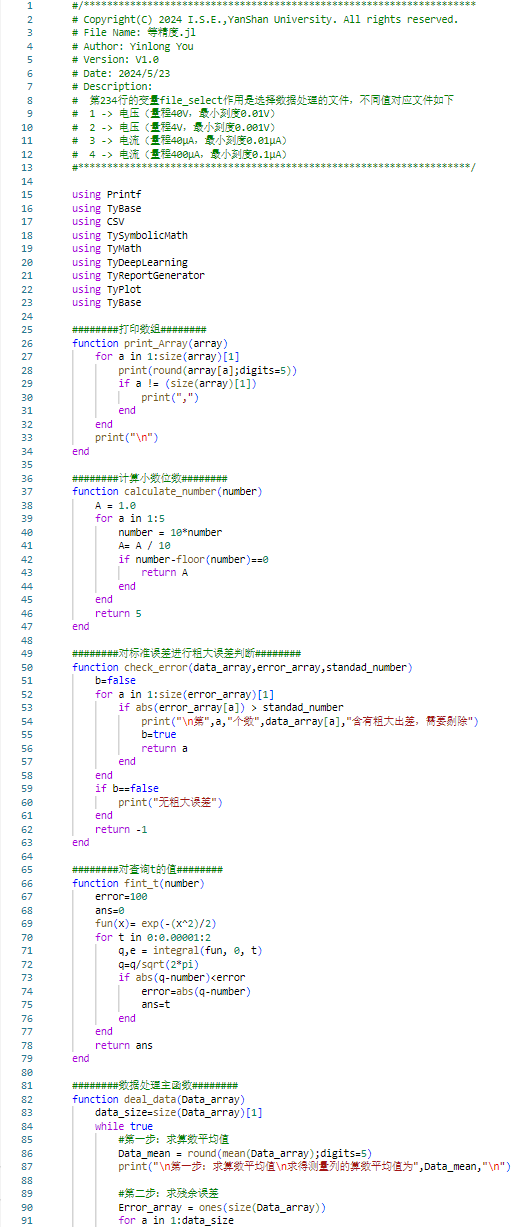
\includegraphics[width=0.9\linewidth]{../截图/等精度处理代码_1}
				\end{subfigure}
				\centering
				\begin{subfigure}{0.325\linewidth}
					\centering
					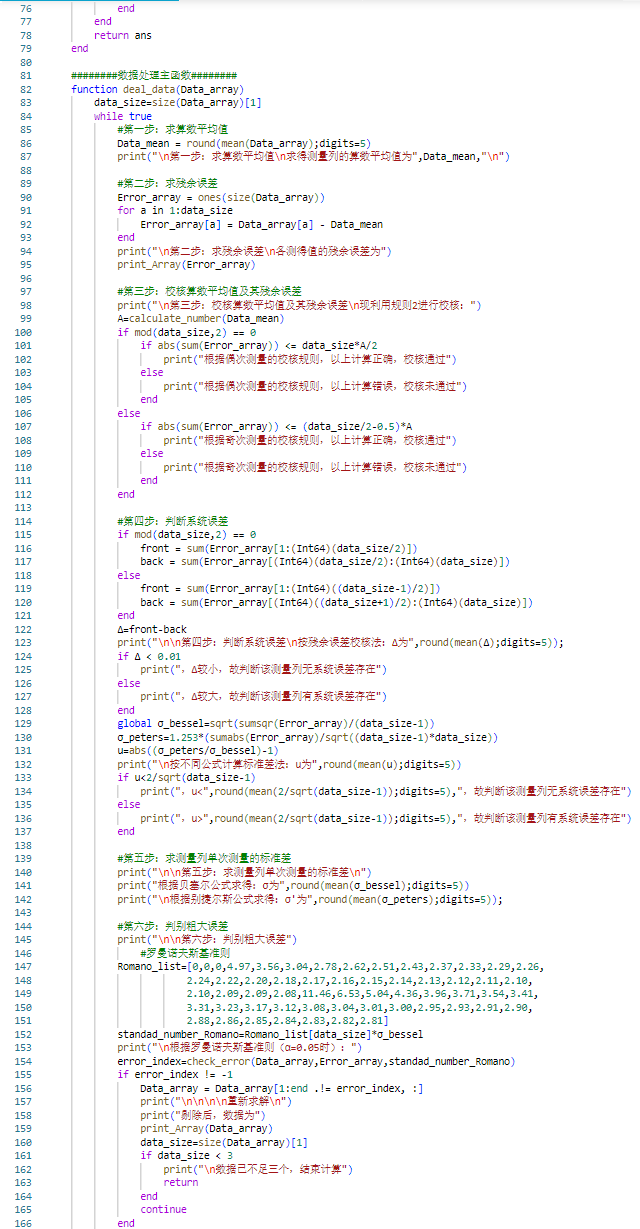
\includegraphics[width=0.9\linewidth]{../截图/等精度处理代码_2}
				\end{subfigure}
				\centering
				\begin{subfigure}{0.325\linewidth}
					\centering
					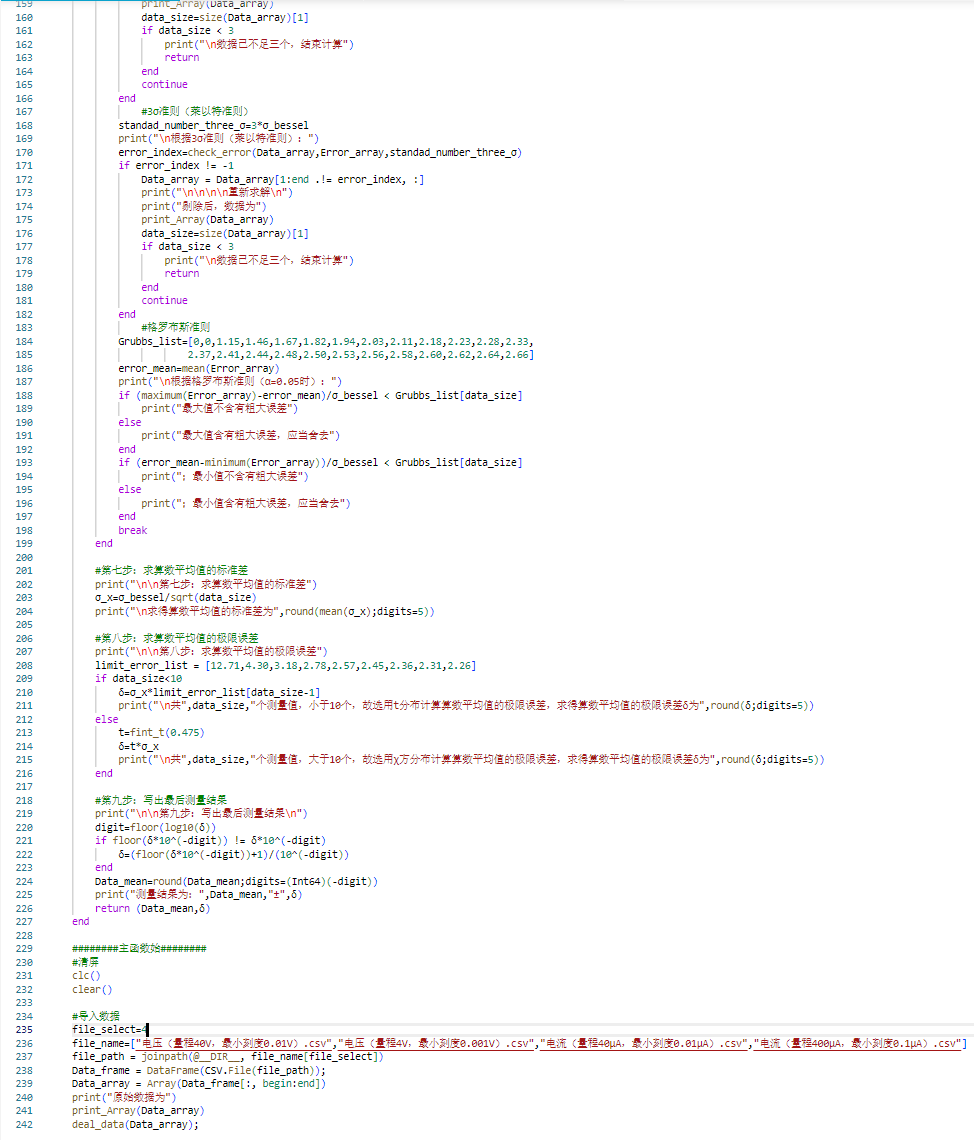
\includegraphics[width=0.9\linewidth]{../截图/等精度处理代码_3}
				\end{subfigure}
				\caption{等精度数据处理代码}
				\label{fig:等精度数据处理代码}
			\end{figure}
			代码流程图如下：
			\begin{figure}[H]
				\centering
				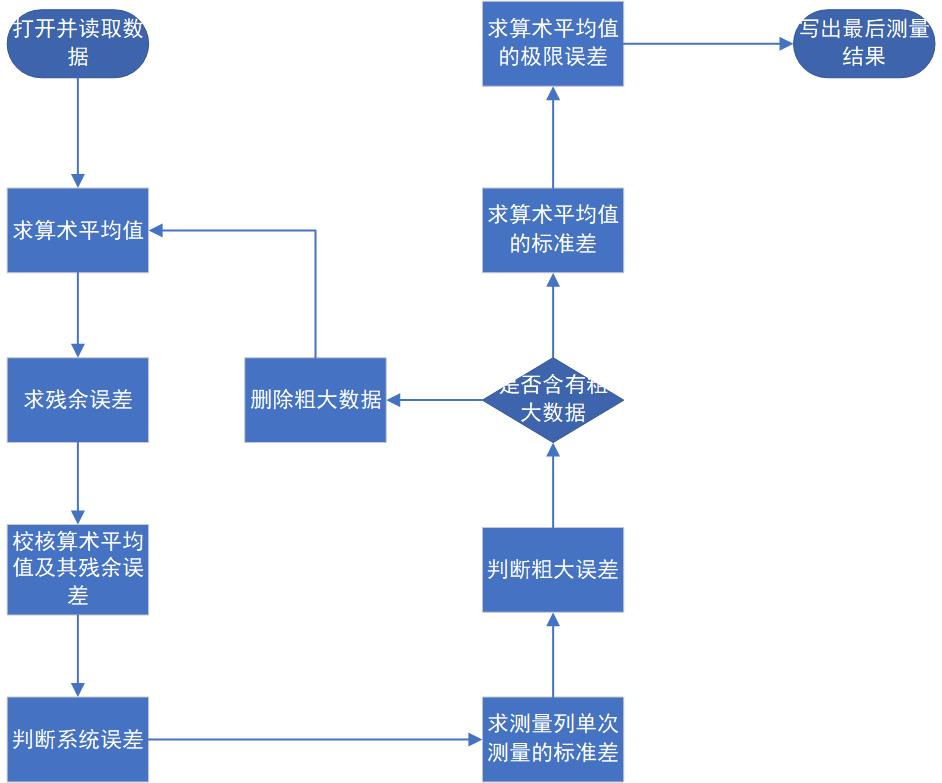
\includegraphics[width=0.45\textwidth]{../截图/等精度流程图}
				\caption{等精度数据处理流程图}
				\label{fig:等精度数据处理流程图}
			\end{figure}
			值得注意的是：
			\begin{compactenum}
				\item 代码可以自动读取数据，并直接根据读取的数据生成对应九个步骤的数据处理操作结果。
				\item 第四步，判断系统误差时，使用了残余误差校核法和不同公式计算标准差法两种方法进行系统误差判断，能更准确的确认系统误差的存在与否。
				\item 第六步，判别粗大误差，使用了罗曼诺夫斯基准则、$3\sigma$准则和格罗布斯准则三种方法进行系统误差判断，能更准确的确认系统误差的存在与否。
				\item 当在第六步确认出现系统误差后，代码可以自行剔除粗大误差数据，并回到第一步重新进行等精度测量。剔除行为直到不存在粗大误差或是数据少于两个时停止。
				\item 第八步，求算术平均值的极限误差时，会根据测量量的个数选择合适、合理的方式进行
				\item 当使用正态分布计算算术平均值的极限误差时，$t$的取值由积分函数反解求得，因此相比于查表法更加精确。
			\end{compactenum}
		\subsection{不等精度数据处理}
			不等精度数据处理按照上述理论写出代码，其代码如图\ref{fig:不等精度数据处理代码}所示
			\begin{figure}[H]
				\centering
				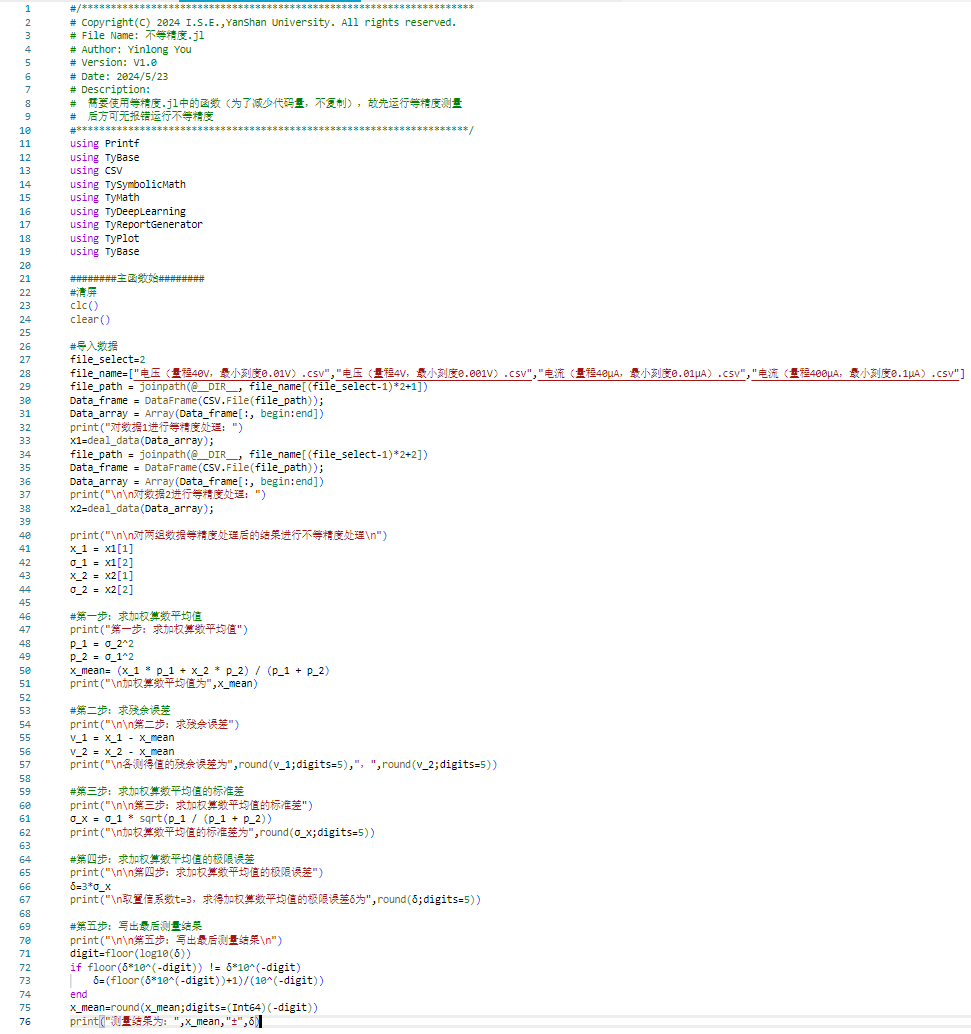
\includegraphics[width=0.45\textwidth]{../截图/不等精度处理代码}
				\caption{不等精度数据处理代码}
				\label{fig:不等精度数据处理代码}
			\end{figure}
			代码流程图如下：
			\begin{figure}[H]
				\centering
				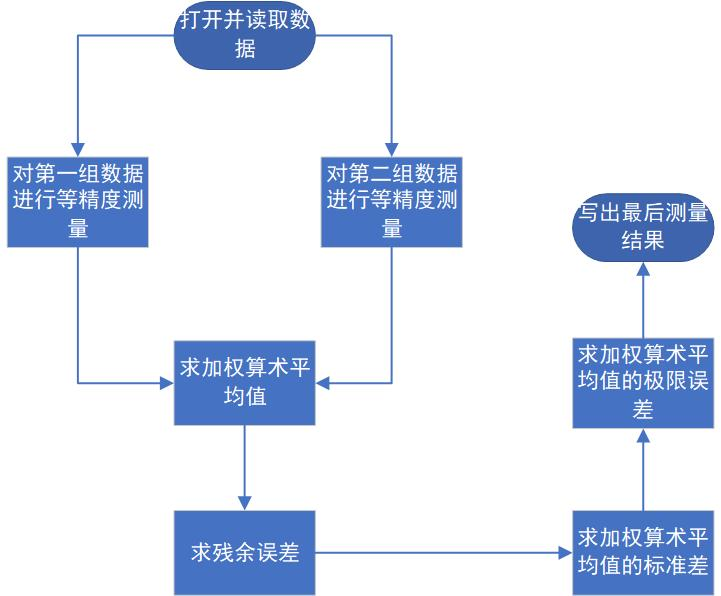
\includegraphics[width=0.45\textwidth]{../截图/不等精度流程图}
				\caption{不等精度数据处理流程图}
				\label{fig:不等精度数据处理流程图}
			\end{figure}
			值得注意的是：
			\begin{compactenum}
				\item 代码可以自动读取数据，并直接根据读取的数据生成对应五个步骤的数据处理操作结果。
				\item 代码首先进行等精度运算，因此可以省去将等精度处理结果复制黏贴到不等精度测量中在进行计算。
			\end{compactenum}
		\subsection{最小二乘法估算}
			最小二乘法估算按照上述理论写出代码，其代码如图\ref{fig:最小二乘法估算代码}所示。由于方程法不适用于电脑计算，因此只采用了矩阵法来计算。\par
			根据测量电路的结构，认为电压表有巨大内阻$R_u$，所以待测电阻$R_x$和一个巨大阻值电阻$R_u$并联，由于$R_u$上的电流远小于$R_x$上的，因此认为$R_u$上的电流恒定为$I_u$，据此有公式：
			$U=(I-I_u)R_x=I R_x-I_u R_x$，其中$U$和$I$为直接测量量，$R_x$和$I_u$为估计量。
			\begin{figure}[H]
				\centering
				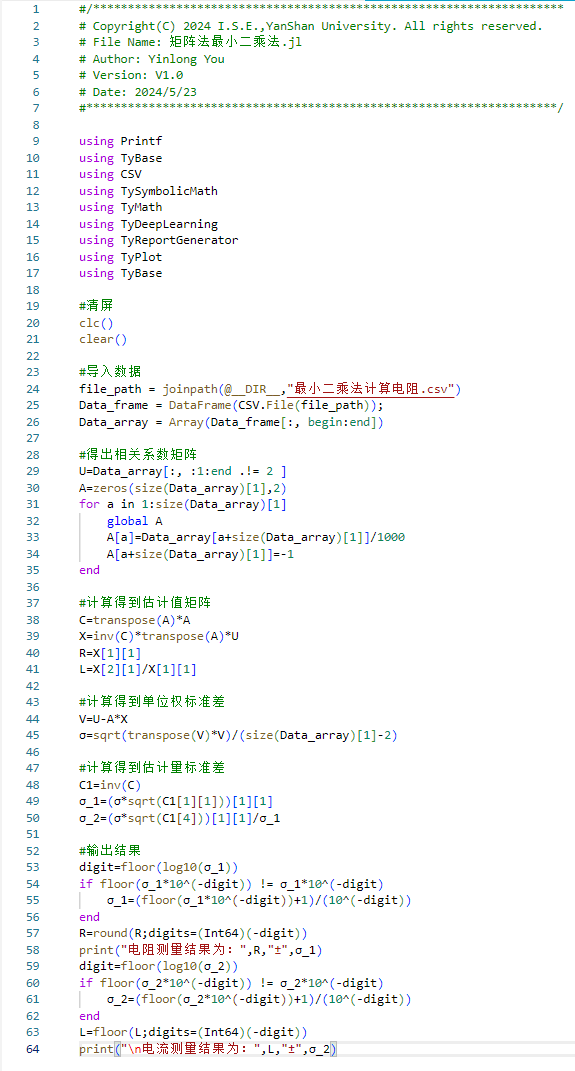
\includegraphics[width=0.34\textwidth]{../截图/最小二乘法回归运算代码}
				\caption{最小二乘法估算代码}
				\label{fig:最小二乘法估算代码}
			\end{figure}
	\section{仿真结果展示}
		由于不等精度数据处理已包含等精度处理，因此以下只展示不等精度数据处理结果和最小二乘法估算结果。
		\subsection{电压不等精度数据处理结果}
			针对电压不等精度数据处理结果如图\ref{fig:电压不等精度处理结果}所示。
			\begin{figure}[H]
				\centering
				\begin{subfigure}{0.325\linewidth}
					\centering
					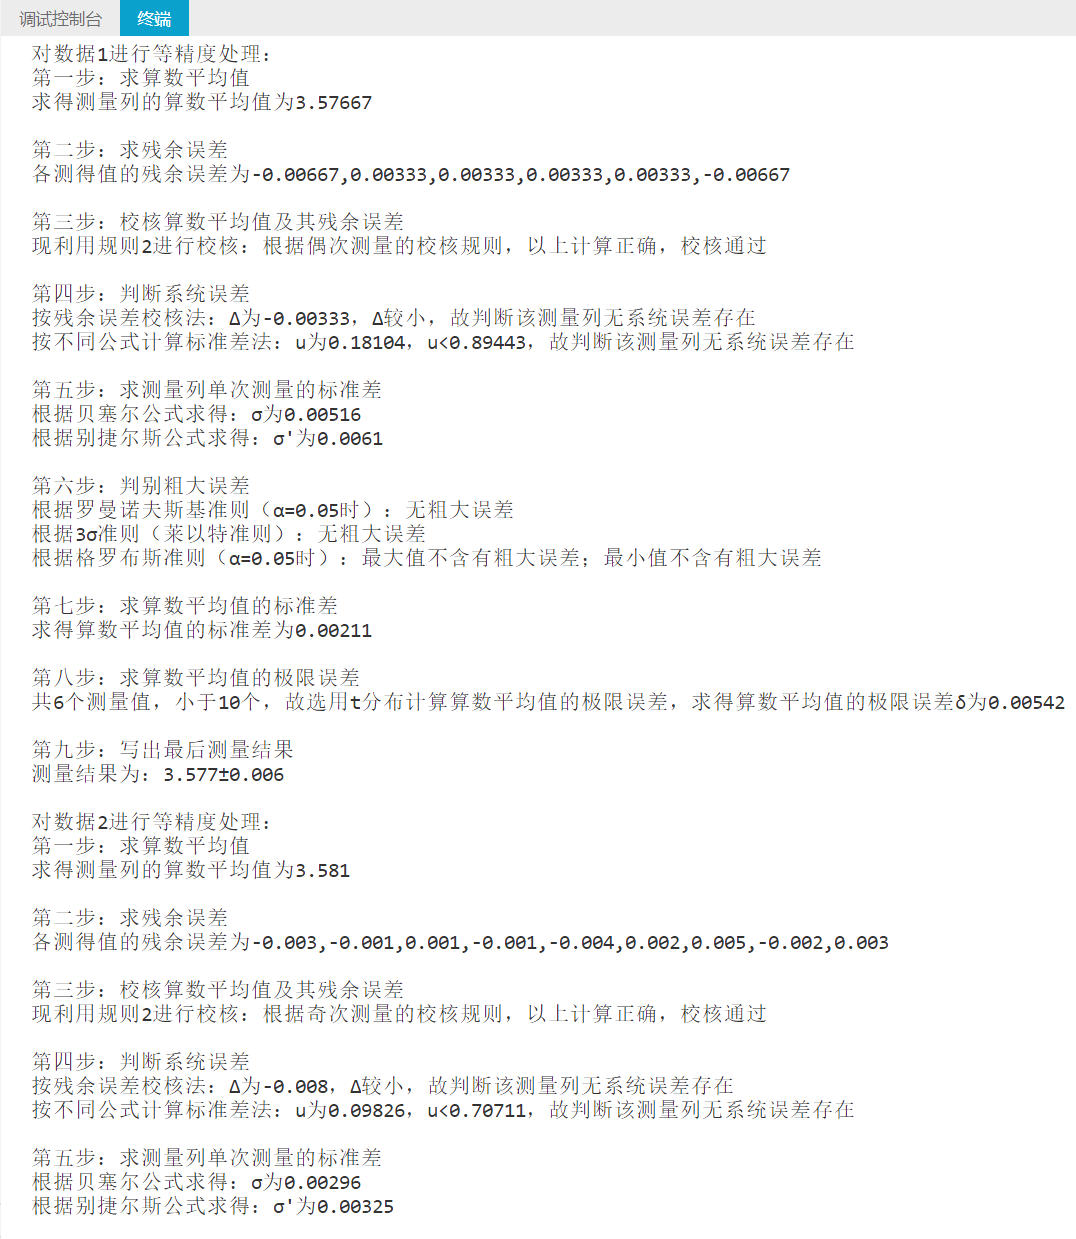
\includegraphics[width=0.9\linewidth]{../截图/电压不等精度处理结果_1}
				\end{subfigure}
				\centering
				\begin{subfigure}{0.325\linewidth}
					\centering
					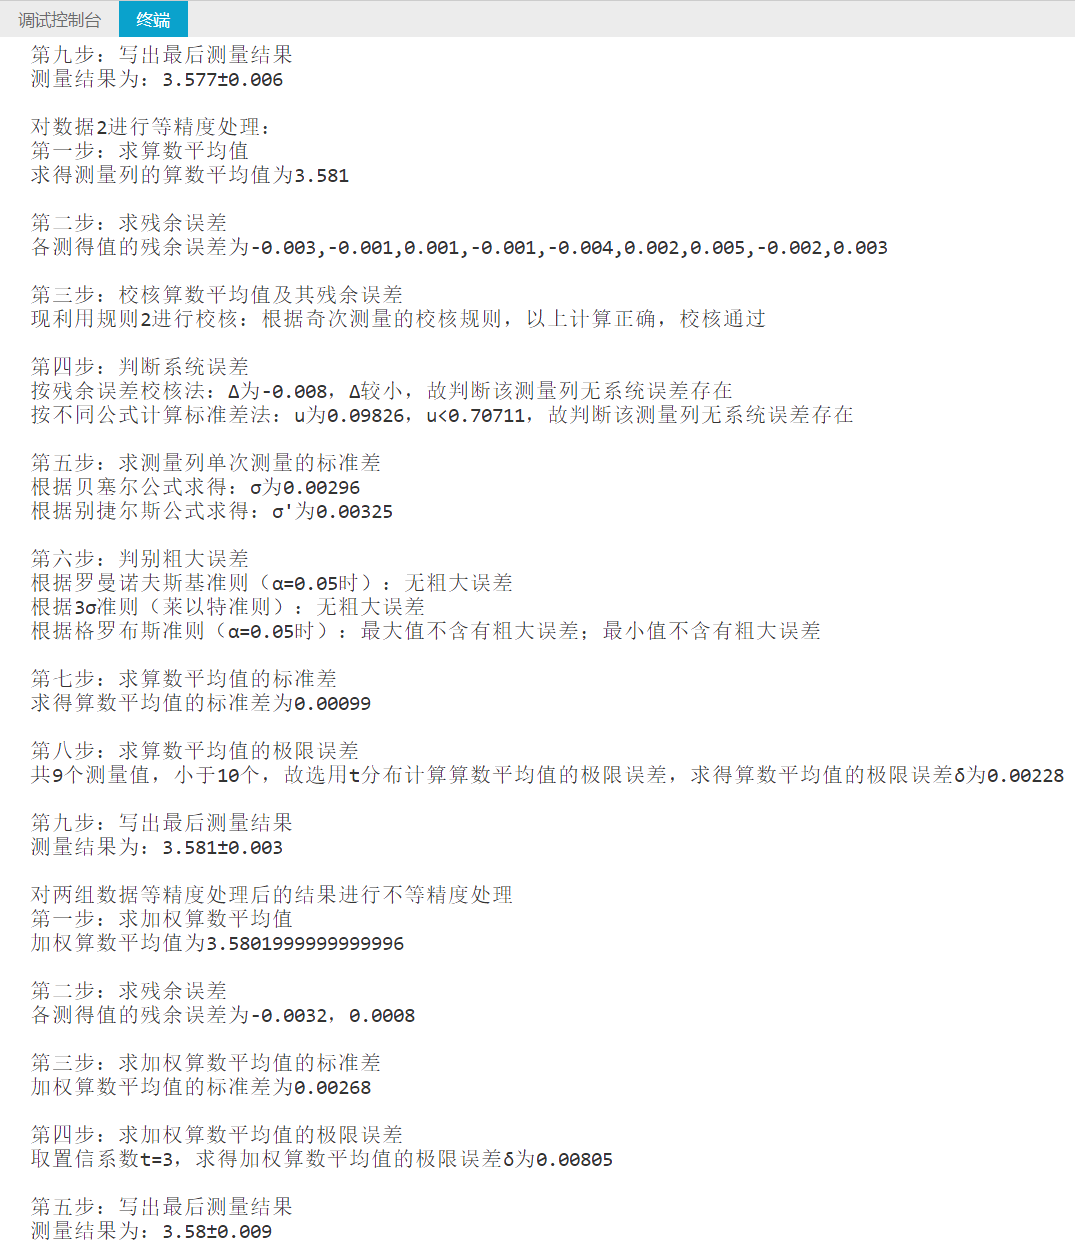
\includegraphics[width=0.9\linewidth]{../截图/电压不等精度处理结果_2}
				\end{subfigure}
				\caption{电压不等精度处理结果}
				\label{fig:电压不等精度处理结果}
			\end{figure}
			根据仿真结果：
			\begin{compactitem}
				\item 表\ref{fig:量程为40V、最小分度值为0.01V时电压采样数据}中的数据不存在系统误差，不存在粗大误差，最终结果为$3.577 \pm 0.006$V
				\item 表\ref{fig:量程为4V、最小分度值为0.001V时电压采样数据}中的数据不存在系统误差，不存在粗大误差，最终结果为$3.581 \pm 0.003$V
				\item 两次结果进行不等精度处理，最终结果$3.580 \pm 0.009$
			\end{compactitem}
		\subsection{电流不等精度数据处理结果}
			针对电流不等精度数据处理结果如图\ref{fig:电流不等精度处理结果}所示。
			\begin{figure}[H]
				\centering
				\begin{subfigure}{0.325\linewidth}
					\centering
					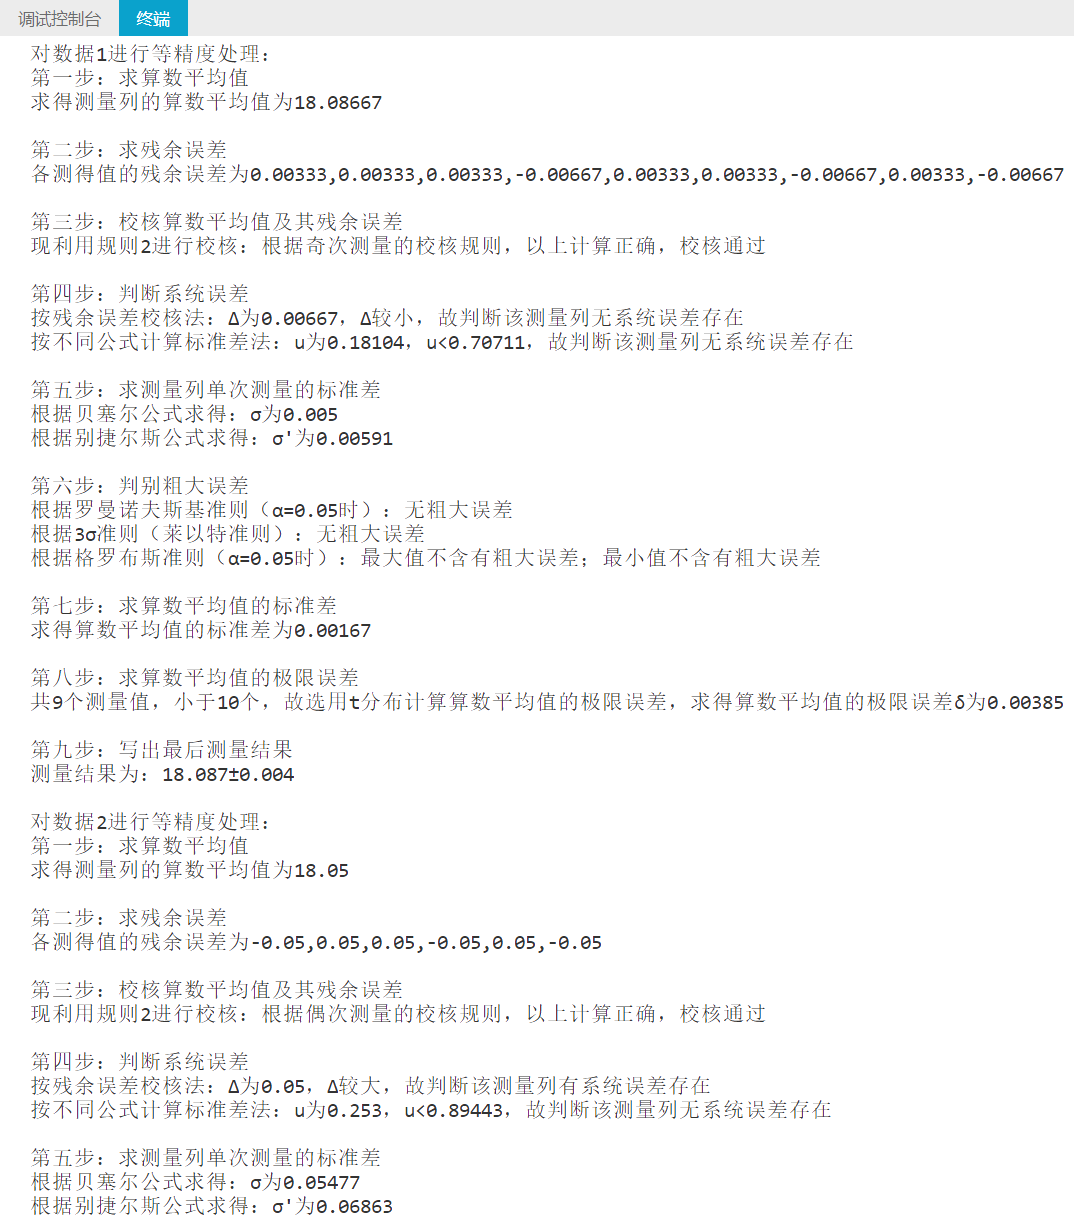
\includegraphics[width=0.9\linewidth]{../截图/电流不等精度处理结果_1}
				\end{subfigure}
				\centering
				\begin{subfigure}{0.325\linewidth}
					\centering
					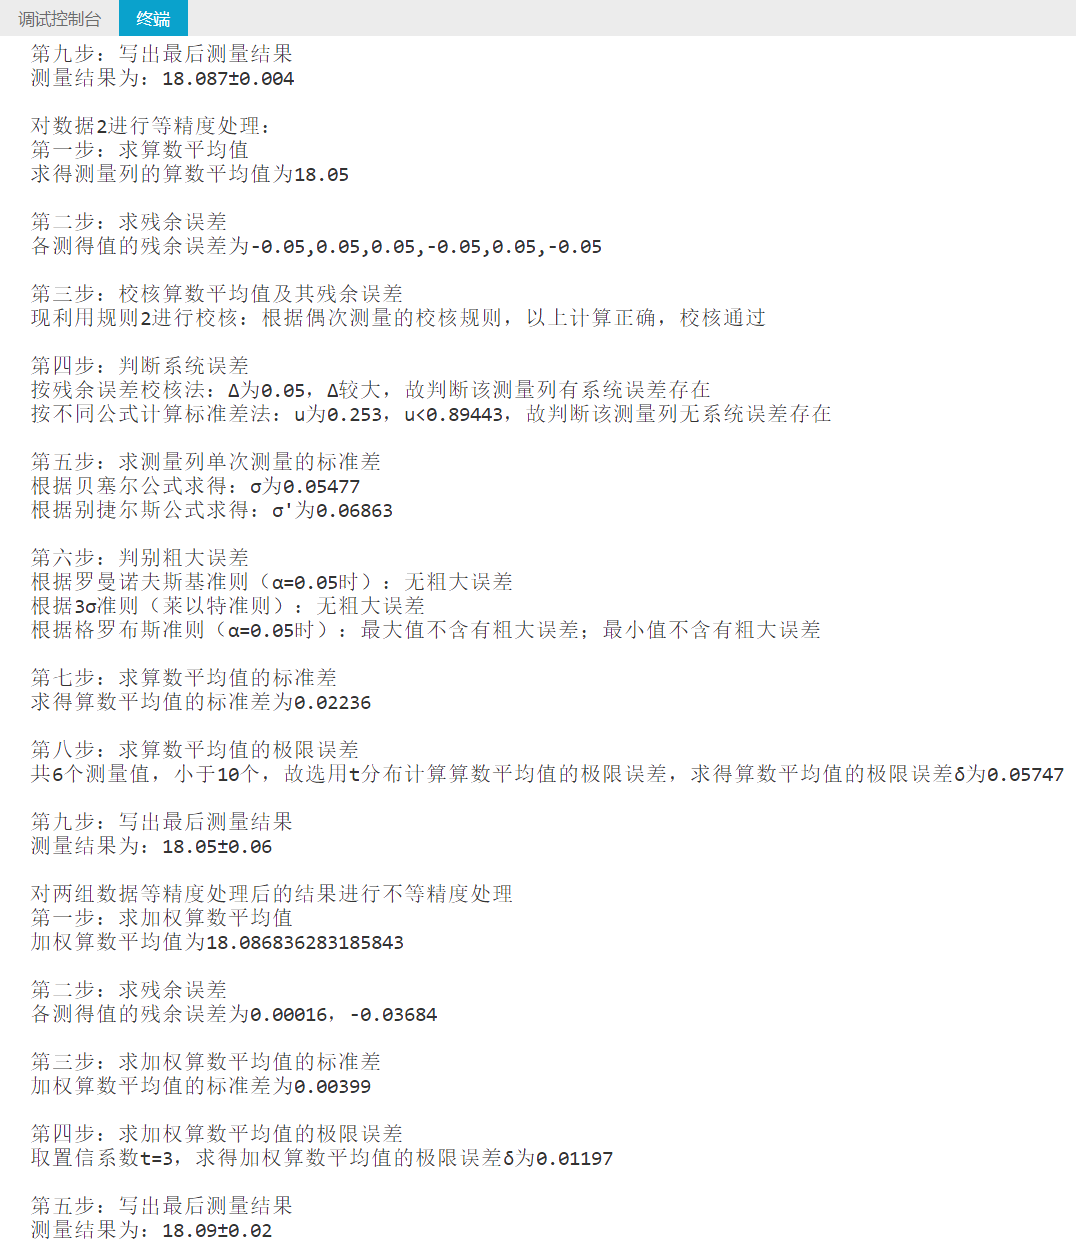
\includegraphics[width=0.9\linewidth]{../截图/电流不等精度处理结果_2}
				\end{subfigure}
				\caption{电流不等精度处理结果}
				\label{fig:电流不等精度处理结果}
			\end{figure}
			根据仿真结果：
			\begin{compactitem}
				\item 表\ref{fig:量程为400uA，最小分度值为0.1uA时电流采样数据}中的数据不存在系统误差，不存在粗大误差，最终结果为$18.05 \pm 0.06\upmu$A
				\item 表\ref{fig:量程为40uA，最小分度值为0.01uA时电流采样数据}中的数据不存在系统误差，不存在粗大误差，最终结果为$18.087 \pm 0.004$
				\item 两次结果进行不等精度处理，最终结果$18.09 \pm 0.02\upmu$A
			\end{compactitem}
		\subsection{最小二乘法估算结果}
			最小二乘法的估计量结果如图\ref{fig:最小二乘法回归运算结果}所示。
			\begin{figure}[H]
				\centering
				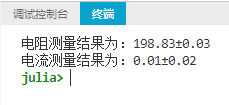
\includegraphics[width=0.34\textwidth]{../截图/最小二乘法回归运算结果}
				\caption{最小二乘法估算结果}
				\label{fig:最小二乘法回归运算结果}
			\end{figure}
			电阻估算结果为:$198.83\pm 0.03$k$\Omega$，根据待测电阻实际的色环为：红黑黑橙棕，可知，电阻实际阻值应该为$200$k$\Omega \pm 1\%=200$k$\Omega \pm 2$k$\Omega$。
			因此证明测量值正确，最小二乘法估算正确。
	\section{结论}
		本文通过误差理论与数据处理的相关手段，对测得电压和电流进行了统计分析，并使用最小二乘法作出了对电阻值的估计。
	
	
	
	
	
	
	
\end{document}